%%%%%%%%%%%%%%%%%%%%%%%%%%%%%%%%%%%%%%%%%
% Masters/Doctoral Thesis 
% LaTeX Template
% Version 1.43 (17/5/14)
%
% This template has been downloaded from:
% http://www.LaTeXTemplates.com
%
% Original authors:
% Steven Gunn 
% http://users.ecs.soton.ac.uk/srg/softwaretools/document/templates/
% and
% Sunil Patel
% http://www.sunilpatel.co.uk/thesis-template/
%
% License:
% CC BY-NC-SA 3.0 (http://creativecommons.org/licenses/by-nc-sa/3.0/)
%
% Note:
% Make sure to edit document variables in the Thesis.cls file
%
%%%%%%%%%%%%%%%%%%%%%%%%%%%%%%%%%%%%%%%%%

%----------------------------------------------------------------------------------------
%	PACKAGES AND OTHER DOCUMENT CONFIGURATIONS
%----------------------------------------------------------------------------------------

\documentclass[11pt, oneside]{Thesis} % The default font size and one-sided printing (no margin offsets)

\graphicspath{{Pictures/}} % Specifies the directory where pictures are stored

\usepackage[square, numbers, comma, sort&compress]{natbib} % Use the natbib reference package - read up on this to edit the reference style; if you want text (e.g. Smith et al., 2012) for the in-text references (instead of numbers), remove 'numbers' 
\hypersetup{urlcolor=blue, colorlinks=true} % Colors hyperlinks in blue - change to black if annoying
\title{\ttitle} % Defines the thesis title - don't touch this

\begin{document}

\frontmatter % Use roman page numbering style (i, ii, iii, iv...) for the pre-content pages

\setstretch{1.3} % Line spacing of 1.3

% Define the page headers using the FancyHdr package and set up for one-sided printing
\fancyhead{} % Clears all page headers and footers
\rhead{\thepage} % Sets the right side header to show the page number
\lhead{} % Clears the left side page header

\pagestyle{fancy} % Finally, use the "fancy" page style to implement the FancyHdr headers

\newcommand{\HRule}{\rule{\linewidth}{0.5mm}} % New command to make the lines in the title page

% PDF meta-data
\hypersetup{pdftitle={\ttitle}}
\hypersetup{pdfsubject=\subjectname}
\hypersetup{pdfauthor=\authornames}
\hypersetup{pdfkeywords=\keywordnames}

%----------------------------------------------------------------------------------------
%	TITLE PAGE
%----------------------------------------------------------------------------------------

\begin{titlepage}
\begin{center}

\textsc{\LARGE \univname}\\[1.5cm] % University name
\textsc{\Large Doctoral Thesis}\\[0.5cm] % Thesis type

\HRule \\[0.4cm] % Horizontal line
{\huge \bfseries \ttitle}\\[0.4cm] % Thesis title
\HRule \\[1.5cm] % Horizontal line
 
\begin{minipage}{0.4\textwidth}
\begin{flushleft} \large
\emph{Author:}\\
\href{http://www.johnsmith.com}{\authornames} % Author name - remove the \href bracket to remove the link
\end{flushleft}
\end{minipage}
\begin{minipage}{0.4\textwidth}
\begin{flushright} \large
\emph{Supervisor:} \\
\href{http://www.jamessmith.com}{\supname} % Supervisor name - remove the \href bracket to remove the link  
\end{flushright}
\end{minipage}\\[3cm]
 
\large \textit{A thesis submitted in fulfilment of the requirements\\ for the degree of \degreename}\\[0.3cm] % University requirement text
\textit{in the}\\[0.4cm]
\groupname\\\deptname\\[2cm] % Research group name and department name
 
{\large \today}\\[4cm] % Date
%\includegraphics{Logo} % University/department logo - uncomment to place it
 
\vfill
\end{center}

\end{titlepage}

%----------------------------------------------------------------------------------------
%	DECLARATION PAGE
%	Your institution may give you a different text to place here
%----------------------------------------------------------------------------------------

\Declaration{

\addtocontents{toc}{\vspace{1em}} % Add a gap in the Contents, for aesthetics

I, \authornames, declare that this thesis titled, '\ttitle' and the work presented in it are my own. I confirm that:

\begin{itemize} 
\item[\tiny{$\blacksquare$}] This work was done wholly or mainly while in candidature for a research degree at this University.
\item[\tiny{$\blacksquare$}] Where any part of this thesis has previously been submitted for a degree or any other qualification at this University or any other institution, this has been clearly stated.
\item[\tiny{$\blacksquare$}] Where I have consulted the published work of others, this is always clearly attributed.
\item[\tiny{$\blacksquare$}] Where I have quoted from the work of others, the source is always given. With the exception of such quotations, this thesis is entirely my own work.
\item[\tiny{$\blacksquare$}] I have acknowledged all main sources of help.
\item[\tiny{$\blacksquare$}] Where the thesis is based on work done by myself jointly with others, I have made clear exactly what was done by others and what I have contributed myself.\\
\end{itemize}
 
Signed:\\
\rule[1em]{25em}{0.5pt} % This prints a line for the signature
 
Date:\\
\rule[1em]{25em}{0.5pt} % This prints a line to write the date
}

\clearpage % Start a new page

%----------------------------------------------------------------------------------------
%	QUOTATION PAGE
%----------------------------------------------------------------------------------------

\pagestyle{empty} % No headers or footers for the following pages

\null\vfill % Add some space to move the quote down the page a bit

\textit{``Thanks to my solid academic training, today I can write hundreds of words on virtually any topic without possessing a shred of information, which is how I got a good job in journalism."}

\begin{flushright}
Dave Barry
\end{flushright}

\vfill\vfill\vfill\vfill\vfill\vfill\null % Add some space at the bottom to position the quote just right

\clearpage % Start a new page

%----------------------------------------------------------------------------------------
%	ABSTRACT PAGE
%----------------------------------------------------------------------------------------

\addtotoc{Abstract} % Add the "Abstract" page entry to the Contents

\abstract{\addtocontents{toc}{\vspace{1em}} % Add a gap in the Contents, for aesthetics

The Thesis Abstract is written here (and usually kept to just this page). The page is kept centered vertically so can expand into the blank space above the title too\ldots
}

\clearpage % Start a new page

%----------------------------------------------------------------------------------------
%	ACKNOWLEDGEMENTS
%----------------------------------------------------------------------------------------

\setstretch{1.3} % Reset the line-spacing to 1.3 for body text (if it has changed)

\acknowledgements{\addtocontents{toc}{\vspace{1em}} % Add a gap in the Contents, for aesthetics

The acknowledgements and the people to thank go here, don't forget to include your project advisor\ldots
}
\clearpage % Start a new page

%----------------------------------------------------------------------------------------
%	LIST OF CONTENTS/FIGURES/TABLES PAGES
%----------------------------------------------------------------------------------------

\pagestyle{fancy} % The page style headers have been "empty" all this time, now use the "fancy" headers as defined before to bring them back

\lhead{\emph{Contents}} % Set the left side page header to "Contents"
\tableofcontents % Write out the Table of Contents

\lhead{\emph{List of Figures}} % Set the left side page header to "List of Figures"
\listoffigures % Write out the List of Figures

\lhead{\emph{List of Tables}} % Set the left side page header to "List of Tables"
\listoftables % Write out the List of Tables

%----------------------------------------------------------------------------------------
%	ABBREVIATIONS
%----------------------------------------------------------------------------------------

\clearpage % Start a new page

\setstretch{1.5} % Set the line spacing to 1.5, this makes the following tables easier to read

\lhead{\emph{Abbreviations}} % Set the left side page header to "Abbreviations"
\listofsymbols{ll} % Include a list of Abbreviations (a table of two columns)
{
\textbf{LAH} & \textbf{L}ist \textbf{A}bbreviations \textbf{H}ere \\
%\textbf{Acronym} & \textbf{W}hat (it) \textbf{S}tands \textbf{F}or \\
}

%----------------------------------------------------------------------------------------
%	PHYSICAL CONSTANTS/OTHER DEFINITIONS
%----------------------------------------------------------------------------------------

\clearpage % Start a new page

\lhead{\emph{Physical Constants}} % Set the left side page header to "Physical Constants"

\listofconstants{lrcl} % Include a list of Physical Constants (a four column table)
{
Speed of Light & $c$ & $=$ & $2.997\ 924\ 58\times10^{8}\ \mbox{ms}^{-\mbox{s}}$ (exact)\\
% Constant Name & Symbol & = & Constant Value (with units) \\
}

%----------------------------------------------------------------------------------------
%	SYMBOLS
%----------------------------------------------------------------------------------------

\clearpage % Start a new page

\lhead{\emph{Symbols}} % Set the left side page header to "Symbols"

\listofnomenclature{lll} % Include a list of Symbols (a three column table)
{
$a$ & distance & m \\
$P$ & power & W (Js$^{-1}$) \\
% Symbol & Name & Unit \\

& & \\ % Gap to separate the Roman symbols from the Greek

$\omega$ & angular frequency & rads$^{-1}$ \\
% Symbol & Name & Unit \\
}

%----------------------------------------------------------------------------------------
%	DEDICATION
%----------------------------------------------------------------------------------------

\setstretch{1.3} % Return the line spacing back to 1.3

\pagestyle{empty} % Page style needs to be empty for this page

\dedicatory{For/Dedicated to/To my\ldots} % Dedication text

\addtocontents{toc}{\vspace{2em}} % Add a gap in the Contents, for aesthetics

%----------------------------------------------------------------------------------------
%	THESIS CONTENT - CHAPTERS
%----------------------------------------------------------------------------------------

\mainmatter % Begin numeric (1,2,3...) page numbering

\pagestyle{fancy} % Return the page headers back to the "fancy" style

% Include the chapters of the thesis as separate files from the Chapters folder
% Uncomment the lines as you write the chapters

% Chapter 1

\chapter{Research} % Main chapter title

\label{Chapter1} % For referencing the chapter elsewhere, use \ref{Chapter1} 

\lhead{Chapter 1. \emph{Research}} % This is for the header on each page - perhaps a shortened title

%----------------------------------------------------------------------------------------

\section{Case Studies}
\subsection{Independent Schools}
\textbf{INDEX Schools} \\
INDEX Schools is a collaboration of over 100 independent schools to ``to share data, analysis, research, and information to aid member schools in decision-making, policy development, and strategic planning" \cite{index}. At the beginning of the 2015 school year, the Assistant Head of Newman emailed the INDEX listserv to request any curriculum outlines or standards and benchmarks for PK-12 computer science that schools might be willing to share. The results of the query are captured in a Google Spreadsheet that can be accessed here: \par

\textbf{Fort Worth Country Day School} \\
Fort Worth Country Day (FWCD) is an independent, coeducational K-12 school in Fort Worth, Texas with a total enrollment of over 1110. Three Newman faculty members toured the school in February of 2016 to observe their CS program. Their Upper School CS sequence progresses as follows: 
\begin{itemize}
	\item 9th: Media Projects or AppInventor
	\item 10th: Art and Code with Processing
	\item 11th: AP CS A with Java
	\item 12th: Data Structures with Java
\end{itemize}
The US uses a block schedule. Classes meet for 75 minutes every other day for one semester. CS courses are treated as general electives, with the exception of “Art and Code,” which satisfies a fine arts credit. \par
There is no US CS requirement at FWCD. Media Projects is currently one section, there are two sections of Art and Code, one section of AP CS, and beginning next year, one section of data structures. With the exception of the introductory course, all CS classes are covered by one faculty member with a computer science background. \par
``Art and Code'' is a prime example of a course that emphasizes the creative capacity of coding. The course is taught in Processing, a visual programming language based on Java that is designed for artists. The teacher, Aaron Cadle, blends his own curriculum with content, labs, and projects developed by Darby Thompson’s, a CS teacher at Sidwell Friends School in Washington D.C. who has developed a project-based introductory CS course. During the observation, Aaron tested student’s understanding of abstract classes using a “Fish Tank” project. Students coded their own interactive, colorful fish that were placed on display in the library, and students outside of the course could vote on their favorite fish. \par
For AP CS Aaron relies on the \href{http://apluscompsci.com/}{A+ Computer Science curriculum}, which includes worksheets, labs, tests, slides, and notes. During the observation, students pulled personally-relevant datasets from data.gov (baseball stats, Powerball numbers, Hilary Clinton emails, etc.) and explored meaningful ways analyze the data using Java (e.g. finding the most common Powerball numbers). Aaron reversed the typical AP structure (lecture in class, worksheets for homework) in order to devote more time to workshopping labs. Students watch short (5 min) instructional videos for homework and work on labs in class. \par
The upper-level CS course, Data Structures, is project based. The course is taught in Java and uses the XBox Kinect. Aaron uses the book, “Making Things See” by Greg Borenstein, which explores the use of Arduinos, Processing, and the Kinect to develop interactive programs. \par
As for Middle School, coding exposure is currently limited to a two week HTML project that is integrated into 7th grade science. A newly hired Middle School iPad Coordinator, brought on to organize the division's one-to-one iPad program, is working to bolster computer literacy across campus. She currently uses 5th and 6th grade advisory time to teach digital citizenship, email etiquette, and Google Classroom. She is also developing curriculum for a required MS technology/computer literacy elective that may be offered next year. When asked about curriculum standards, she pointed to ISTE benchmarks. \par
Lower School computer science exposure at FWCD is very similar to Newman's. A ``Computer Special" offered to grades K-4 meets for 40 minutes every 1 out of 6 days. The class takes place in the ``lab" - a proto-makerspace/ design thinking workshopping space. The special explores engineering exercises, programmable hardware (Sphero, LittleBits, Lego robotics, etc.), and coding (ScratchJr and Kodable). FWCD has never taught keyboarding; instead they direct interested parents/students to online resources. At one point the computer teacher, Mandy Lofquist, maintained a ``technology checklist" of all the computing skills her students should acquire, although she hasn't relied on this list since her students started coding. \par


\textbf{Greenhill} \\
Greenhill School, a PK-12 coeducational private day school outside of Dallas, Texas, has an enrollment over 1200. This is another school that Newman faculty members toured in February, 2016 to observe their curriculum and classrooms. The Director of Technology, Chris Bigenho, has been researching computer science programs and developing K-12 CS curriculum for the last five years. Emphasis on aligning the program across divisions and with national standards has led to the current implementation, which is one of the more advanced programs in the INDEX schools consortium. \par 
The Upper School CS program is a three-tier, two year sequence. Students may take multiple courses from each tier (each a semester long course). There is a 1 trimester CS graduation requirement. The courses include:
\begin{itemize} 
	\item CS1: Introduction to CS with Arduino
	\item CS1: Beginning JAVA Programming 
	\item CS1: Introduction to Game Design 
	\item CS1: Engineering
	\item CS2: Advanced Computational Design
	\item CS2: Intermediate JAVA Programming
	\item CS3: Advanced Topics in Computer (prepares students for AP)
\end{itemize}
Greenhill’s Middle School courses are broken into trimesters and rotate every 6 days. Classes meet for approximately 50 minutes. One block of the schedule is split between two electives; each meets every other day corresponding to ACE or BDF blocks. Band and choir may meet during ACE the entire year, while 2D or 3D art meets for a single semester during BDF. \par
Greenhill offers two required electives, ``Exploratory Design,'' that blend coding (Scratch, Arduino) with engineering design challenges. An example project includes prototyping, 3D printing, and testing a hub and blades for a wind turbine. The coding sequence is as follows:
\begin{itemize}
	\item 5th grade - Exploratory Design (required)
	\item 6th grade - Exploratory Design (required)
	\item 7th/8th grade - Prototyping 1 (optional elective)
	\item 7th/8th grade - Prototyping 2 (proposed optional elective)
	\item 7th/8th grade - Game Design (proposed optional elective)
\end{itemize}
After Exploratory Design, the electives are no longer required. Prototyping I is an optional 7th and 8th grade “arts” elective that meets every other day for one trimester. Students work through “Arduino Projects,” a project book of 10+ exercises that introduce Arduino, servos, LEDs, and other simple circuits. \par
Now that Greenhill has an introductory CS course at the US level, the plan (discussed by both the MS head and the director of technology) is to consider making a CS course required in 7th and 8th grades. \par
The LS exposure takes place in 2nd - 4th grades in Computer 2, 3, and 4. These courses are a mix of computer literacy and coding (Microworlds), which is likely to change now that the computer teacher is retiring.

\subsection{Public High Schools}
Examining the top fifteen public high STEM schools, as ranked by the U.S. News in 2015 \cite{usnews}, provides insight into the state of computer science in some of the nation's top STEM high schools. Roughly 3/4th of the list's top 15 schools offered at least one CS course, significantly more than the national average cited by Gallup of 1 in 4 U.S. schools \cite{gallup}. About half of these schools offered a basic (no requirement, strictly elective) computer science sequence: an introductory CS course (frequently in Java), followed by the AP CS course. Four of the 15 schools had a robust, scaffolded CS sequence; these schools are examined below. \par
\textbf{Thomas Jefferson High School for Science and Technology} \\
Thomas Jefferson High School for Science and Technology (TJ) is ranked \#2 on U.S. News' STEM report. A ``regional Governor's school" in Virginia with 1,846 enrolled students, TJ offers five years of Computer Science. There is a one credit CS graduation requirement that ``most students satisfy by taking Foundations of Computer Science in 9th grade during the summer" \cite{tjreq}. Additional courses (\href{https://www.tjhsst.edu/research-academics/math-cs/computer-science/docs/FlowCS1516.pdf}{the sequence for which can be found on their website}) include: AP Computer Science and Data Structures, Artificial Intelligence 1 \& 2, Parallel Computing 1 \& 2, Mobile App Development, Web App Development, and Mobile/Web Application Development Lab.\par
Thomas Jefferson HS's overall graduation requirements are listed in Table \ref{tjtable}. Computer science courses, including the graduation requirement, fall under ``electives." It's important to note that TJ's graduation requirements are largely similar to Newman's. \par
\begin{table}[]
\centering
\caption{Thomas Jefferson High School Graduation Requirements \cite{tjreq}}
\label{tjtable}
\begin{tabular}{lc}
\textbf{Subject}       & \textbf{Required Credits} \\ \hline
English                & 4                     \\
Math                   & 4                     \\
Science                & 4                     \\
History/Social Studies & 4                     \\
World Language         & 3                     \\
Health/PE              & 2                     \\
Fine Arts              & 1                     \\
Economics/Personal Finance              & 1                     \\ 
Electives              & 3                     \\
\textbf{Total}         & \textbf{26}          
\end{tabular}
\end{table}
\textbf{Stuyvesant High School} \\
Stuyvesant High School, a nationally-ranked New York City public high school with 3,285 students, ranked 14th on the U.S. News' top STEM schools. Stuyvesant offers 6 active CS courses that are listed through the math department. Although none of the CS courses satisfy the 4-sequence math requirement, students are required to take a single semester ``Introduction to Computer Science." In the introductory course, 
\begin{blockquote}``Students will study some the basic themes and subfields of computer science including algorithms and programming, simulation, networking, computability, graphics, and artificial intelligence. Students will also be given a solid foundation in working in a modern networked computer environment. This is a required course beginning with the Class of 2007. Students will take the course either in the Fall or Spring term of their sophomore year" \cite{stuy}.
\end{blockquote} 
Additional CS courses offered to high school students include: AP Computer Science, System Level Programming, Computer Graphics, Software Development, and Computer Science Intel Research. \par
\textbf{High Technology High School} \\
High Technology High School (HTHS) in Lincroft, New Jersey, has an enrollment of 280 and is ranked \#1 in U.S. News' top STEM schools. HTHS is relatively unique for its strong integration of technology and programming into engineering courses. CS courses include: Computer Programming for Engineers, Computer Science \& Software Engineering, and Digital Electronics \cite{hths}. \par
\textbf{Edison Academy for Science, Mathematics, and Engineering Technologies} \\
The Academy for Science, Mathematics, and Engineering Technologies, a magnet school located in Edison, New Jersey, has a total enrollment of 161 students and is ranked \#4 in the U.S. News top STEM public high schools \cite{usnews}. \par
The high school operates on a rotating block schedule; all classes meet Monday for one period, and classes meet on either Tuesdy/Thursday or Wednesday/Friday for two periods (88 minutes). Engineering courses, however, meet every day of the week. Students enroll in either the ``civil and mechanical" or ``electronics and computer engineering" track. The requirements for the Electronics and Computer Engineering Technology (ECET) Program are listed in Table \ref{ecet}. \par
 \begin{table}[]
 \centering
 \caption{Edison Academy: Electronics and Computer Engineering Technology (ECET) Program of Study \cite{edisonacad}}
 \label{ecet}
 \begin{tabular}{|l|l|}
 \hline
 \multirow{4}{*}{9}  & Introduction to Engineering  \\ \cline{2-2} 
                     & Introduction to Digital Logic \\ \cline{2-2} 
                     & Introduction to Computer Science Using C++  \\ \cline{2-2} 
                     & DC Circuit Analysis \\ \hline
 \multirow{5}{*}{10} & Integrated Circuit Logic Families  \\ \cline{2-2} 
                     & Sequential Logic Circuits \\ \cline{2-2} 
                     & Finite State Machines (FSM) \\ \cline{2-2} 
                     & Interfacing to the analog world \\ \cline{2-2} 
                     & Microcontrollers / Assembly language \\ \hline
 \multirow{4}{*}{11} & Object Oriented Programming Using C++  \\ \cline{2-2} 
                     & AC Circuit Analysis \\ \cline{2-2} 
                     & Electronic Communication Systems \\ \cline{2-2} 
                     & Digital Communication Systems \\ \hline
 \multirow{2}{*}{12} & Senior Project \\ \cline{2-2} 
                     & Programming with JAVA \\ \hline
 \end{tabular}
 \end{table}
 %---------------------
\textbf{Westside Magnet High School for Integrated Technology} \\
Although Westside Magnet High School for Integrated Technology, did not make U.S. News' list of top 15 public STEM schools, its robust CS program warrants attention. The magnet school in Houston, Texas, gives students the option to choose one of five strands in business, computing sciences and engineering, fine arts, health science and technology, or media. The school reportedly uses the four year engineering curriculum developed by \href{https://www.pltw.org/}{Project Lead the Way} \cite{westside}. \par
Students who choose the Computing Sciences and Engineering strand choose between one of three programs: Computer Programming, Computer Maintenance, and Engineering. Each program is an individually designed; a typical four year schedule is detailed in Table \ref{westsidesched}. ``Magnet courses" (specific to the Computing Sciences and Engineering strand) are outlined in Table \ref{westsidemag}. 
\begin{table}[]
\centering
\caption{Four Year Plan for Westside HS Computing Sciences and Engineering \cite{westside}}
\label{westsidesched}
\begin{tabular}{|l|l|l|l|}
	 \hline
\textbf{9th}     & \textbf{10th}        & \textbf{11th}         & \textbf{12th}               \\ \hline
English          & English              & AP Language           & AP Literature               \\ \hline
Algebra/Geometry & Geometry/ Algebra II & Alga. II/Pre-Calculus & Pre-Calculus/Calculus       \\ \hline
World Geography/ & World History        & U S History           & Go/Economics                \\ \hline
Biology          & Chemistry            & Physics               & AP Science/Elective Science \\ \hline
Foreign Language & Foreign Language     & Foreign Language      & Health/Speech               \\ \hline
\rowcolor[HTML]{FFCC67} Magnet Course   & Magnet Course        & Magnet Course         & Magnet Course   \\ \hline
Fine Arts Credit & PE                   & Elective              & Elective					  \\ \hline                   
\end{tabular}
\end{table}


\begin{table}[]
	\centering
	\footnotesize
	\caption{Westside HS Computing Sciences and Engineering Magnet Courses \cite{westside}}
	\label{westsidemag}
	\begin{tabular}{|p{3.5cm}|p{3.5cm}|p{3.5cm}|p{3.5cm}|}
		\hline
	\textbf{9th}     & \textbf{10th}        & \textbf{11th}         & \textbf{12th}               \\ \hline
Principles of Information Technology/ Principles of Art, A/V Technology and Communication & Pre-AP Computer Science 1 (Python) or Computer Progamming & Pre-AP Computer Science 2 (JAVA) or Pre-AP Computer Science 1 (Python) & AP Computer Science 1 (JAVA) or Pre-AP Computer Science 2 (JAVA) \\ \hline
Principles of Information Technology/ Principles of Art, A/V Technology and Communication & Computer Maintenance & Telecommunications and Networking & Research and IT Solutions or Practicum in Business Management    \\\hline
Introduction to engineering Design & Principles of Engineering & Digital Electronics & Engineering Drafting and Design \\\hline
Concepts of Engineering & Robotics & Principles of Technology & Engineering Mathematics \\ \hline                                    \end{tabular}
\end{table}

\subsection{Higher Education}
Preparation for college is obviously paramount in any Upper School academic program at Newman, and so it's instructive to examine the range of CS courses and subjects offered in higher education. 
\textbf{MIT} \\
Massachusetts Institue for Technology is a consistently top-ranked, globally-recognized leader in education, research, and innovation. MIT's Electrical Engineering and Computer Science (EECS) Department is the largest department at MIT and is composed of four undergraduate degree programs: Electrical Science and Engineering, Electrical Eng. \& Computer Science, Computer Science and Engineering, and Computer Science and Molecular Biology. All four tracks are required to take EECS I, an introductory electrical engineering and computer science course:
\begin{blockquote}
\textbf{6.01 Introduction to EECS I} - An integrated introduction to electrical engineering and computer science, taught using substantial laboratory experiments with mobile robots. Key issues in the design of engineered artifacts operating in the natural world: measuring and modeling system behaviors; assessing errors in sensors and effectors; specifying tasks; designing solutions based on analytical and computational models; planning, executing, and evaluating experimental tests of performance; refining models and designs. Issues addressed in the context of computer programs, control systems, probabilistic inference problems, circuits and transducers, which all play important roles in achieving robust operation of a large variety of engineered systems \cite{mit}.
\end{blockquote}
There is a close link between electrical engineering and computer science throughout MIT's undergraduate CS program. Thanks to tools like Arduinos, Raspberry Pis, VEX and LEGO robotics, and other easily-programmed microcontrollers, it's possible to develop Upper School curriculum that explores computer science through an electrical or mechanical engineering lens. As for CS fundamentals, MIT's more traditional introductory CS course is described below:
\begin{blockquote}
	\textbf{6.S04 Special Subject: Fundamentals of Programming} - Introduces fundamental concepts of programming. Designed to develop skills in applying basic methods from programming languages to abstract problems. Topics include programming and Python basics, computational concepts, software engineering, algorithmic techniques, data types, and recursion and tail recursion. Lab component will consist of software design, construction and implementation of design \cite{mit}. 
	\end{blockquote} \par
\textbf{Pomona College} \\
Pomona College, a small liberal arts college in Claremont, California, offers the perspective of a top-tier post-secondary school without an engineering department. CSCI051 is the first course in the CS sequence, and it specifies that no previous programming experience is required.
\begin{blockquote}
	\textbf{CSI051} - Introduction to the field of computer science using the object-oriented language Java. Topics include iteration and recursion, basic data structures, sorting and searching, elementary analysis of algorithms and a thorough introduction to object-oriented programming. Special emphasis on graphics, animation, event-driven programming and the use of concurrency to make more interesting programs  \cite{pomonacs1}. 
\end{blockquote}
CSCI052, the second course in the introductory series, emphasizes ``functional programming, procedural and data abstraction, recursion and problem-solving" as well as ``computer architecture and organization, finite automata and computability" \cite{pomonacs1}. These subjects are closely aligned with the CSTA benchmarks for upper level computer science.  \par 
The following goals of the Pomona CS major have been pulled from the department's website: \cite{pomona}
\begin{enumerate}
	\item To conceptualize multiple views of problems, to develop computational solutions grounded in theory, and to evaluate their solutions using a range of metrics.
	\item To work alone and in teams to identify, formulate, and solve computing problems.
	\item To gain a firm grounding in the core areas of computer science: theory, systems, programming languages, and algorithms.
	\item To apply the knowledge gained in core courses to a broad range of advanced topics in computer science, and to develop the ability to learn sophisticated technical material independently.
	\item To be able to communicate technical information both orally and in writing.
	\item To understand the theoretical, practical, and ethical ramifications of computational solutions to problems, and to be aware of current research developments in computer science.
\end{enumerate}

\section{National Standards}
\subsection{CSTA}
The Computer Science Teachers Association (CSTA) released the revised ``K-12 Computer Science Standards" in 2011, which is widely cited in the computer science education community as source of CS benchmarks. The CSTA outlines a set of learning objectives on three levels and grouped into one of five ``strands": computational thinking; collaboration; computing practice; computers and communication devices; and community, global, and ethical impacts \cite{csta}. The benchmarks begin at the elementary level and continue through high school. AP CS curriculum fits well into the level 3 CSTA sequence, but CSTA recommends additional CS courses for depth. For the list of standards, refer to Appendix \ref{AppendixCSTA}.\par
\subsection{ISTE}
The International Society for Technology in Education (ISTE) has compiled a set of standards for computer science educators \cite{iste}. These standards are listed in Appendix \ref{AppendixISTE} and are cross-referenced with CSTA benchmarks. Unlike CSTA, ISTE does not describe K-12 standards, but rather outlines a set of learning objectives that could presumably be covered in one or more advanced high school courses. When mapped to the CSTA benchmarks, ISTE standards mostly fall under level 3A (at the AP CS level) are are not particularly useful for identifying the requirements for introductory curriculum. In addition to computer science concepts, these standards layout teaching standards and strategies specific to educators and learning environments. \par
\subsection{College Board's Advanced Placement}
Since 2003 the \href{http://media.collegeboard.com/digitalServices/pdf/ap/ap-course-overviews/ap-computer-science-a-course-overview.pdf}{Advanced Placement Computer Science A} exam has tested students' ability to solve problems and design algorithms using Java. The College Board's test is intended to cover the equivalent of a first semester college computer science course. The topics include:
\begin{enumerate}
	\item Object-Oriented Program Design:  Program and class design 
	\item Program Implementation: Implementation techniques. Programming constructs, Java library classes
	\item Program Analysis: Testing, Debugging, Runtime exceptions, Program correctness, Algorithm analysis
	\item Standard Data Structures:  Primitive data types, Strings, Classes, Lists, Arrays (1-D and 2-D) 
	\item Standard Operations and Algorithms: Searching, Sorting
	\item Computing in Context: System reliability, Privacy, Legal issues and intellectual property, Social and ethical ramifications of computer use 
\end{enumerate}
In 2016 the College Board plans to release a second AP CS course, \href{https://secure-media.collegeboard.org/digitalServices/pdf/ap/ap-computer-science-principles-curriculum-framework.pdf}{AP Computer Science Principles}, that will operate in tandem to the other AP CS class. From the AP website, ``AP Computer Science Principles offers a multidisciplinary approach to teaching the underlying principles of computation." Unlike the AP CS A which relies exclusively on Java, the Principles course allows teachers to use any programming language. The course introduces key programming concepts with a ``focus on fostering students to be creative." The ``Big Ideas" covered by this exam include:
\begin{enumerate}
	\item Creativity
	\item Abstraction
	\item Data and Information
	\item Algorithms
	\item Programming
	\item Internet
	\item Global Impact
\end{enumerate} \par
\begin{table}
	\centering
	\bgroup
	\def\arraystretch{1.5}
	\begin{tabular}{ p{7cm} p{7cm} }
		\hline
		\textbf{AP Computer Science \textit{A}} &	\textbf{AP Computer Science \textit{Principles}} \\ \hline \hline
		\multicolumn{2}{l}{\textit{Curriculum:}} \\
		Focused on object-oriented programming and problem solving & Built around fundamentals of computing including problem solving, working with data, understanding the Internet, cybersecurity, and programming. \\ \hline
		\multicolumn{2}{l}{\textit{Language:}} \\
		Java is the designated programming language	& Teachers choose the programming language(s) \\ \hline
		\multicolumn{2}{l}{\textit{Skillset:}} \\
		Encourages skill development among students considering a career in computer science or other STEM fields & Encourages a broader participation in the study of computer science and other STEM fields, including AP Computer Science A \\ \hline
		\multicolumn{2}{l}{\textit{Assessment:}} \\
		Multiple-choice and free-response questions (written exam) & Two performance tasks students complete during the course to demonstrate the skills they have developed (administered by the teacher; students submit digital artifacts), and multiple-choice questions (written exam) \\ \hline
	\end{tabular}
	\egroup 
	\caption{Comparison of AP Computer Science Exams ~\cite{APcomp}} \label{tab:apexams} 
\end{table}\par
For a detailed list of learning benchmarks associated with this exam, \href{https://secure-media.collegeboard.org/digitalServices/pdf/ap/ap-computer-science-principles-curriculum-framework.pdf}{check out the AP Computer Science Principles Curriculum Framework}. \par

\textbf{PROS \& CONS OF AP CS} \\
There are merits and shortcomings of teaching Advanced Placement courses in general, as well as those that are specific to computer science. Given the 
Perhaps the most salient advantage is the potential for college credit, which may allow students to place out of introductory-level college courses and save time or money in higher education. AP courses may also positively affect college transcripts since AP courses at Newman are weighted in the student’s cumulative GPA calculation. In addition, because College Board is an internationally-recognized organization, there is a thriving community willing to offer support or share resources, curriculum, example labs, and exercises. Finally, the AP course offers a set of well-researched standards and benchmarks that, at in theory, align with equivalent college-level courses. \par
It's unclear how the AP designation might affect CS course enrollment at Newman. On the one hand, high-achieving students who might typically take AP Biology or Chemistry electives may be more likely to take AP CS since it would offer the same GPA and transcript distinctions as other AP science or math courses. On the other hand, students with a passion for computer science but with a less rigourous course load might shy away from an advanced CS course as a result of the AP distinction. Another alternative- offering an AP caliber course that prepares students for an optional AP exam at the end of the semester- may cater to both groups of students. Ultimately, student feedback is necessary to determine the best course of action to maximize enrolloment. \par
Cons AP A
Java, although many colleges use this language
It comes with a ton of paradigm baggage ("Ms deBB, what does public static void main(String[] args) mean?"
have to spend the first week just getting Eclipse or IntelliJ installed.
Java, and thus the AP course limit students to the kinds of programming that can be expressed in Java. It's a rigid, enterprisy way to do things.
Plus, you'd have to spend a ton of time practicing for the test.
Not creative
Inflexible - With a course you design yourself, you can recruit the best students regardless of background, and mold the curriculum to fit their needs and interests
Not project based
Cons AP Principles
 Still young, early; 
How will colleges respond? Is it adequate preparation for college level CS?



\subsection{Next Generation Science Standards}
The Next Generation Science Standards (NGSS) is the product of twenty-six states and broad-based teams working to develop a new set of science standards needed to revise a 15-year-old set of documents on which most state standards are based \cite{ngsss}. Unfortunately, the latest NGSS document does not enumerate standards specific to computer science, for the reasons explained below:
\begin{blockquote}
``Computer Science and Statistics Computer science and statistics are other areas of science that are not addressed here, even though they have a valid presence in K-12 education... Computer science, too, can be seen as a branch of the mathematical sciences, as well as having some elements of engineering. But, again, because this area of the curriculum has a history and a teaching corps that are generally distinct from those of the sciences, the committee has not taken this domain as part of our charge. Once again, this omission should not be interpreted to mean that computer science or statistics should be excluded from the K-12 curriculum. There are aspects of computational and statistical thinking that must be understood and applied in learning about the sciences, and we identify these aspects, along with mathematical thinking, in our discussion of science practices in Chapter 3" \cite{ngsss}. 
\end{blockquote}\par
Although the NGSS does not explicitly outline CS benchmarks, the Engineering Design standards are highly applicable to software engineering or computational thinking projects. These benchmarks are covered in Appendix \ref{AppendixNGSS}. \par
For CS courses that are not standalone but rather are integrated into existing math or science classes, aligning curriculum with relevant NGSS standards may be advisable. Code.org has published two sets of middle school curriculum- CS in Algebra and CS in Science- that are consistent with both CSTA and NGSS standards. A table summarizing the overlap between these standards as it relates to this curriculum can be \href{https://code.org/curriculum/science}{found on their website}.

\section{Online Curriculum}
A non-exhaustive list of online coding tools and curriculum can be found in Appendix \ref{AppendixTools}. Tools are separated by level (lower, middle, and upper school). The table contains information about professional development, platform cost, student tracking, and the possibility for self-guided online learning. \par 
At the elementary school level, iPad apps (Kodable) and drag-and-drop visual programming languages (Hopscotch, Scratch, SNAP!, Tynker) teach foundational coding concepts through interactive games, art, and animations. Many of these platforms cater to teachers without computer science experience. For example, Tynker includes assessment, classroom management, lesson plans, and a built in tutor. In addition, Tynker aligns to Common Core Mathematics, Common Core ELA, and CSTA Computer Science standards \cite{tynker}. \par
Many of the elementary-level tools (Scratch, Tynker, SNAP!) can be used in more sophistocated projects at the middle school level. For integrating CS into existing middle school courses, Code.org provides 20-lesson CS in Algebra and CS in Science modules, as well as in-person or online professional development. \par
The upper school curriculum typically focuses on exploring computer science concepts with a true development language (Java, Javascript, Python, etc.). CodeAcademy and Kahn Academy use videos and cloud-coding to deliver instruction in a variety of languages, including Javascript, Ruby, Python, and more. Online AP Computer Science courses are available through CodeHS and Edhesive, each of which offer PD and student tracking.  \par

\textbf{ONLINE VS. CLASSROOM INSTRUCTION} \\

\section{Hardware Tools}
Physical coding platforms open the door to a variety of highly-engaging ways to teach coding to all ages. Robotics, wearable tech, electronic music, and interactive games are just a few examples of potential projects that can be used to teach coding or computational thinking. Please refer to Appendix \ref{AppendixHardware} for a table of tools.
%% Chapter Template

\chapter{Newman Past and Present} % Main chapter title

\label{Chapter2} % Change X to a consecutive number; for referencing this chapter elsewhere, use \ref{ChapterX}

\lhead{Chapter 2. \emph{Newman Past and Present}} % Change X to a consecutive number; this is for the header on each page - perhaps a shortened title


%----------------------------------------------------------------------------------------
\section{Previous Programs}
The inclusion, dissolution, and subsequent reemergence of computer science in secondary education is not unique to Newman. As Kafai and Burke ~\cite{backtoschool} point out, in the 1980s many schools featured Basic or Logo programming, but by the mid 90s, CS was on the decline. Kafai and Burke point to the lack of subject-matter integration, difficulty finding qualified instructors, and rise of the internet precipitating a shift of emphasis from programming to software-specific proficiency and web surfing literacy. They argue that several significant changes, such as the plethora of fun and engaging coding sites with self-guided, online curriculum, are responsible for a resurgance in CS education. In addition, they point to ``a shift from tools to communities." Sites like Scratch operates much like a social networking site that facilitates content sharing and open source exchange \cite{backtoschool}.



\section{Present Status}
% LOWER SCHOOL -------------------------------------------
\subsection{Lower School}
\textbf{Coding Already Happening} \par
Exposure to coding in Lower School currently takes place during Media. Susie Toso meets with grades 1-4 once per week for 50 minutes. 
\begin{definition}
\item [2nd] Code.org
\item [3rd] Scratch
\item [4th] Computer literacy: keyboarding (Typing Pal, which is currently the perview of the homeroom; 2x week for 10 minutes)
\end{definition}
Jennifer Williams and Elaine Sevin offer a collaborative 2nd/5th grade LEGO WeDo robotics unit that meets once per month for 50 minutes. The excerise, to control a soccer player and kick a ball into a LEGO goal, simulates real life phenonmenon through LEGOs and code. Students are introduced to CS topics such as abstraction, problem deconstruction, and serialization of tasks. While this robotics exposure is a valuable and highly-engaging engineering exercise that clearly augments LS coding curriculum, additional time is required to convey foundational CS topics. \par
Finally, programmable hardware is used in 2nd grade science. During the Mars unit, students program Bee-Bots, small robots for teaching sequencing and problem solving. \par

\textbf{LS Faculty Brainstorm} \par
A facilitated brainstorm during an afternoon faculty meeting helped to elicit thoughts and concerns from all Lower School teachers regarding both computer literacy and coding. Faculty divided into groups based on a grade and answered the following questions on Post-its: \par
\begin{definition}
	\item [Q1.] How is technology used in your classroom?
\item [Q2.] What do you wish/ think your students should know that they currently don't about coding and computer literacy?
\item [Q3.] What are your hopes and dreams for computing? 
\item [Q4.] What are your concerns about implementing coding curriculum at Newman?
\end{definition}
A table of all of the responses can be found in Appendix [insert]. There were a handful of recurring ideas that emerged across all grades. LS teachers were concerned about the balance of coding vs. computer literacy, specifically that the rise of coding came at the cost of students' ability to effectively operate computers in class. Additional proficiency and knowledge of word processing, internet research, internet safety and ethics, file structure, keyboarding, and troubleshooting were some of the most common responses to questions two and three. \par
As for question four - concerns related specifically to implenting coding curriculum - teachers overwhelmingly cited the need for CS professional development. The issue of time was also raised multiple times: how will CS fit into the existing schedule, and what will be sacraficed to make room for this new subject? \par

\textbf{Meeting Benchmarks} \par
The CSTA benchmarks, found in Appendix \ref{AppendixCSTA}, are the most highly cited and comprehensive CS standards, especially for grades K-6. Many of the CSTA benchmarks are already met by Newman's existing curriculum. Discussed below are coding and computer literacy benchmarks less likely to be covered by default. \par
In grades K-2, CSTA places emphasis on computer literacy, multimedia exposure, and computational thinking. The ability to break large problems into discrete steps, to think sequentially, and to sort information are the core of the coding/computational thinking standards. The computer literacy benchmarks are perhaps more vague - to effectively use computer input/output devices and conduct research an in age-appropriate way. \par
Selected CSTA K-2 benchmarks:
\begin{definition}
	\item [CODING]
	\item [L0CP04]	Construct a set of statements to be acted out to accomplish a simple task (e.g., turtle instructions).  
	\item [L0CT02]	Use writing tools, digital cameras, and drawing tools to illustrate thoughts, ideas, and stories in a step-by-step manner.
	\item [L0CT03]	Understand how to arrange (sort) information into useful order, such as sorting students by birth date, without using a computer.
	\item [COMPUTER LITERACY]
	\item [L0CD01]	Use standard input and output devices to successfully operate computers and related technologies.
	\item [L0CP01]	Use technology resources to conduct age-appropriate research.
\end{definition}
In grades 3-6, coding standards include the ability to implement problem solutions using block-based programming like Scratch, to understand and develop simple algorithms, and to break up larger problems into sub-problems. Computer literacy standards echo many subjects that arose during the LS brainstorm: proficiency with word processing, email, keyboarding, troubleshooting, internet safety and ethics, and web searching. \par 
Selected CSTA standards for grades 3-6:
\begin{definition}
	\item [CODING]
	\item [L1CP05]	Construct a program as a set of step-by-step instructions to be acted out.
	\item [L1CP06]	Implement problem solutions using a blockbased visual programming language. 
	\item [L1CT01]	Understand and use the basic steps in algorithmic problem-solving (e.g., problem statement and exploration, examination of sample instances, design, implementation, and testing).
	\item [L1CT02]	Develop a simple understanding of an algorithm (e.g., search, sequence of events, or sorting) using computer-free exercises.
	\item [L1CT05]	Make a list of sub-problems to consider while addressing a larger problem.
	\item [COMPUTER LITERACY] 
	\item [L1C01]	Use productivity technology tools (e.g., word processing, spreadsheet, presentation software) for individual and collaborative writing, communication, and publishing activities. 
	\item [L1C02]	Use online resources (e.g., email, online discussions, collaborative web environments) to participate in collaborative problemsolving activities for the purpose of developing solutions or products.
	\item [L1CD1]	Demonstrate an appropriate level of proficiency with keyboards and other input and output devices
	\item [L1CD3]	Apply strategies for identifying simple hardware and software problems that may occur during use.
	\item [L1CI01]	Discuss basic issues related to responsible use of technology and information, and the consequences of inappropriate use.
	\item [L1CI02]	Identify the impact of technology (e.g., social networking, cyber bullying, mobile computing and communication, web technologies, cyber security, and virtualization) on personal life and society.
	\item [L1CI03]	Evaluate the accuracy, relevance, appropriateness, comprehensiveness, and biases that occur in electronic information sources.
	\item [L1CI04]	Understand ethical issues that relate to computers and networks (e.g., equity of access, security, privacy, copyright, and intellectual property).
	\item [L1CP04]	Gather and manipulate data using a variety of digital tools.
	\item [L1CP08]	Navigate between webpages using hyperlinks and conduct simple searches using search engines. 
\end{definition}
At this point in time, LS Newman curriculum is on track to meet the CSTA standards. Specific program recommendations are discussed in the next section.\par
% UPPER SCHOOL -------------------------------------------   
US \par

As of writing, CS exposure at Newman is largely self-guided and limited to a small group of students. Approximately 5 students are enrolled in Online Global Academy, an online platform offering courses in a variety of subject areas. The CS courses include: 
% http://www.globalonlineacademy.org/the-goa-experience/courses/
\begin{itemize}
\item Art of Code: Processing
\item Computer Programming I: Computational Thinking
\item Computer Programming I: Java
\item Computer Programming II: Advanced Java
\item Computer Programming II: Analyzing Data with Python
\item Computer Programming II: iOS Development
\end{itemize}

Students in Tech Club meet on a weekly basis to build and program their autonomous drone. Coding Club ostensibly engaged students in extracurricular CS, although, like many student groups, participation quickly waned as students got bored with online exercises. Several other students cite summer coding programs or online platforms like Kahn Academy for exposure to programming languages like Python and C++. Although a small handful of students are finding time and ways to code, Newman's Upper School is not providing adequate opportunities to develop critical foundational CS skills, nor is it reaching an adequate portion of the student body.  \par

Greg Malis, an US math teacher, argues that computer science fits into both science and math: ``What we do in math is explore patterns, algorithms, and there is no more concrete version of an algorithm than code." As for science: ``It fits. The ultimate goal of science is to formulate hypotheses, test, and debug. That, in a nutshell, is what coding's about." When asked about the role of computer science in K-12 education, Malis responded: ``Our job is to prepare students. If our students graduate without any exposure to coding, we aren't doing our job."

 
%% Chapter Template

\chapter{Recommendations} % Main chapter title

\label{Chapter3} % Change X to a consecutive number; for referencing this chapter elsewhere, use \ref{ChapterX}

\lhead{Chapter 3. \emph{Recommendations}} % Change X to a consecutive number; this is for the header on each page - perhaps a shortened title


%----------------------------------------------------------------------------------------
\section{Lower School}
\section{Middle School}
Possible implementation strategies to explore: CS integrated in the classroom, 6th grade science course, club time, flex time, new schedule

\section{Upper School}
Unlike the Middle School schedule, the Upper School sequence affords time and space for computer science electives, and potentially a graduation requirement. The rotating eight block schedule means there are 32 possible credits, although Newman students rarely graduate with greater than 30, typically averaging approximately 27 credits. The student handbook stipulates that students must complete 24 academic credits to graduate, taken from the following subject areas: \par

\begin{table}
	\begin{center}
\begin{tabular}{ | l | c | }
	
	\hline
	\textbf{Subject} & \textbf{Credits} \\ \hline
	English & 4 \\ \hline
	Mathematics & 4 \\ \hline
	History/Social Studies & 4 \\ \hline
	Science & 3 \\ \hline
	World Languages & 3 \\ \hline
	Arts & 2 \\ \hline
	Physical Education & 2 \\ \hline
	Electives & 2 \\ \hline
	\textbf{Total} & \textbf{24} \\ \hline
\end{tabular} 
\caption{Upper School Graduation Requirements} \label{tab:usreqs} 
\end{center}
\end{table}
\par
The ``elective" graduation requirement is the most obvious space to insert CS courses. It's worth examining which departments and classes may be impacted by these additional electives.\par
If the ultimate objective is to treat CS as foundational subject on par with core subjects like math and English, a critical analysis of the Upper School curriculum will be required to make space for a new set of mandated credits. Given the nascent status of computer science at Newman, this document will not attempt to evaluate the merits of the existing sequence or propose potentially subversive structural changes. Nevertheless, it's instructive to examine schools with robust CS requirements and evaluate how a similar program at Newman might affect existing courses.\par


\hiddensubsection{Standards}

\hiddensubsection{AP Computer Science}
For a full analysis of the pros and cons of AP Computer Science, please refer to %TODO. 
This document strongly recommends against offering AP Computer Science A, especially as a first entry into CS, because of the curriculum's rigidity, lack of creativity, and use of the Java programming language; however, for a select group of students, typically those with existing CS experience and a strong committment to the subject, an independent study or online course like CodeHS may be advisable. This AP does not have broad appeal and is not ideal for inspiring students; it is, however, both rigorous and aligned to many college-level courses. \par
AP Computer Science Principles, on the other hand, may offer both the national recognition of an AP while still preserving the creative and innovative component of CS. This new AP is young, so time and experimentation may be necessary to determine the course's true value. Offering AP CS Principles (or an equivalent but unaccredited course that prepares students for success on the AP) as a second or third tier, year-long course is recommended.\par


\hiddensubsection{Online Education}
For a full analysis of online platforms, their merits and shortcomings, please refer to %TODO.
There are several examples where online programs add clear value to Newman's CS offerings. Allowing platforms like Global Online Academy or CodeHS to fill niche needs- such as allowing self-directed students to take specific upper level courses- is cost-effective and grants students more options. In addition, using Kahn Academy or other online resources as a crutch or supplement may bolster in-class instruction.\par
This document, however, does not recommend the strict reliance on online CS platforms, especially for meeting a potential graduation requirement. By the very nature of being ``cookie cutter'' and purely virtual, online platforms cannot offer the same ``rigor and relationships'' as curriculum spearheaded by a teacher. Hooking students, inspiring students, communicating the importance and broad applicability of CS, and ensuring that students recognize the creative and innovative potential of coding- these must be the priorities of a CS program at Newman. Without the enthusiasm and relationships created by and with teachers, the personally-relevant and curated projects, or the hands-on communication, students will be less likely to pursue or take interest in CS.\par 
To summarize: the human element is the value added by independent school education. Newman is known for its top-notch pedagogy; CS, a critically important field in the 21st century, cannot be the exception. \par
All of that said, hooking students is the priority, after which students may want more freedom to explore advanced topics on their own. Using online CS programs as a second or third tier course may be advisable, but only if resources or hiring difficulties prohibit an in-person CS experience. \par   

\hiddensubsection{Stage 1}


\hiddensubsection{Stage 2} 
\hiddensubsection{Stage 3}
\hiddensubsection{CS Graduation Requirement} \par
This document strongly recommends that the Upper School adopts a 1/2 credit CS graduation requirement. A mandated credit, as opposed to an optional elective, ensures that every student- especially groups typically underrepresented in CS- get exposure to coding prior to college. \par


- staffing requirements \par
- space requirements \par
%% Chapter Template

\chapter{Recommendations} % Main chapter title

\label{Chapter4} % Change X to a consecutive number; for referencing this chapter elsewhere, use \ref{ChapterX}

\lhead{Chapter 4. \emph{Recommendations}} % Change X to a consecutive number; this is for the header on each page - perhaps a shortened title

A table of K-12 CS benchmarks tailored specifically for Newman can be found in Appendix \ref{AppendixNEWMAN}. These benchmarks were compiled using frameworks and curriculum from the CSTA (Appendix \ref{AppendixCSTA}), ISTE (Appendix \ref{AppendixISTE}), Computing at School (Appendix \ref{AppendixCOMP}), College Board (Section \ref{CBAP}), universities, code schools, and other online resources. \par
It felt necessary to tailor benchmarks specifically for Newman given some of the shortcomings of existing standards. CSTA benchmarks are narrowly specific in some subject areas, overly vague in others, or excessively pedantic (e.g. ``use technology to conduct age-appropriate research''). ISTE and the College Board's AP are restrictive in their sole focus on upper school. By picking from and refining established benchmarks, the list enumerated in Appendix \ref{AppendixNEWMAN} hopes to provide a concise but thorough set of standards that can be used as the bedrock framework for an aligned, K-12 CS program at Newman.
%----------------------------------------------------------------------------------------
\section{Lower School}
It is exciting to report that Media and LS science currently address the coding benchmarks outlined in Appendix \ref{AppendixNEWMAN}. The following recommendations explore potential ways improve upon the current program.\par 
Using Media time to explore physical computing may help reach a group of students that responds well to tactile instruction. Robotics also serves to introduce engineering at an early age, in addition to reinforcing CS concepts learned through online coding platforms. Hardware programming occurs in 2nd and 5th grade science through Bee-Bots or LEGO WeDo, but time with these technologies is limited and could be augmented by Media. Unfortunately, Susie Toso reports that the Media block is barely enough time to get students logged in and coding; adding hardware only complicates setup time. The need for funding or additional professional development may be another barrier to physical computing.\par
Kodable is currently one of the main online platforms used to teach coding in the LS, and so a critical evaluation of its strengths and weaknesses should inform its use in the classroom. One of the issues with Kodable is that many of the lessons follow the same format; there is little variability within units (``Loopy Lagoon,'' ``Condition Canyon,'' etc.). While repetition helps to reinforce concepts, the formulaic exercises may develop high proficiency with the game without developing a foundational understanding of the underlying skill.\par 
Another potential weakness of the platform is that it does not visually reinforce terms; the absense of text labels (``functions,'' ``loops,'', etc.) may be an intentional design decision to accommodate new readers, but developing a coding vernacular is an important step towards identifying themes and ideas across CS. On the plus side, the accompanying lesson plans are very thorough and outline solid learning objectives that teachers can use to reinforce concepts (e.g. ``functions help recycle code so there are no repeats''). That said, these teacher resources are dense and could be confusing, particularly for teachers who may be new to CS. Distilling these lesson plans down in a way that is digestible for the intended audience, K-5 students, may not be straight-forward.\par
\par
The section Asteroidia is perhaps the most problematic section, which calls into question the validity of the platform as a whole. As an experienced programmer, I struggled to determine how the exercise (shooting asteroids) was linked to a computer science concept; after reading the teacher resource, I can say that the link between shooting asteroids and variable assignment is tenuous as best. In general, I found the section to be little more than an overly complex, confusing shooting game with unclear numbers and letters, all of which were supposed to communicate variables, Strings, and Ints.\par
The important takeaway from this section, a point that is relevant to any lower school coding platform, is that the underlying concepts and learning objectives should match the age-appropriate benchmarks enumerated in Appendix \ref{AppendixNEWMAN}. Kodable tries to cover middle and upper school subjects in its K-5 platform, with mixed results. Variables (the core learning objective of the aforementioned Asteroidia section) are not a recommended benchmark until middle school because students have not explored this relatively complex subject in math classes. The same goes for Strings, Ints, arrays, and classes (subjects explored in Kodable lessons). Early exposure is certainly not detrimental, and in some cases may be advantageous, but in the case of Kodable, attempting to present advanced material resulted in a confusing asteroid game. Sticking to K-5 benchmarks is likely a better use of coding time, as additional emphasis on loops, sequences, conditional statements, and functions will lay a foundation for future advanced CS coursework.\par 
All of these criticisms aside, Kodable is still a good resources for PK-2 coding. The sections on sequencing, problem decomposition, loops, conditionals, and functions clearly communicate ideas through fun, engaging exercises. By providing additional context to help students identify recurring ideas and themes, which Susie is already doing, and exposing students to additional coding platforms (currently the case), Kodable can be considered one of several tools in the early education coding toolbox.\par
The other heavily-used platform, Code.org, currently offers a series of impressive online courses. Unlike Kodable, lessons are variegated, and there is opportunity for free play (as opposed to exercises with a single solution). The online curriculum also includes ``unplugged'' activities, activities that don't require a computer, which is another way to actively engage students in a hands-on experience of CS. In addition, the ability to ``see code'' may allow curious students to get an early taste of text-based coding, the step beyond block-based programming. Videos from diverse professionals in the field help to communicate at an early age who codes (Women! People of color!) and what coding entails.\par

Another issue that may be worth exploring is the gap in the LS CS sequence since 5th graders currently do not take Media. Since Susie Toso currently works part-time, she would not be able to cover 5th grade even if there were space in the schedule. The other gap (PK and K) is not as concerning. While coding exercises and platforms exist at this age, there are a limited number of benchmarks to be covered at the lower school level, and beginning before 1st grade may not be a valuable use of time.  \par
As illustrated in the LS faculty brainstorm (Appendix \ref{AppendixBRAIN}), there may be \textit{computer literacy} benchmarks, in addition to coding benchmarks, that should be articulated and addressed. While these topics should not necessarily be the purview of Media, establishing a list of computer literacy benchmarks to be distributed between technology, the library, and the classroom may help to ensure that students don't fall through the cracks, as well as help establish clear expectations between teachers. With the hiring of a new LS librarian, this is an opportune time to develop library curriculum that meets some of these computer literacy benchmarks. Conducting internet research, safely using the internet, and creating word processing documents could be just a few examples of important computer-related topics that do not need to take up coding time. Finally, keyboarding is another important computer literacy skill that is covered by classroom teachers. Examining the efficacy of this program (and debating the overall necessity of mandated keyboarding) should be explored by LS teachers and administrators. \par
One final recommendation is to consider a capstone coding project or assessment prior to 6th grade.  This type of project may help to ensure all students are on the same page upon entering middle school. Many online platforms offer assessment tools, but an open-ended Scratch project, for example, could be a more creative way to demonstrate mastery.\par
Oskie Creech, the coordinator of Design Thinking and Innovation at Newman, suggested the possibility of a final coding project in 5th grade. He currently sees all 5th graders for design thinking and said that one semester could be devoted to coding. Since coding lends itself nicely to open-ended design problems and since there is currently a CS gap in 5th grade, his class may be an optimal place in which to implementing a capstone coding project.\par 
\hiddensubsection{Summary}
To summarize, Susie Toso has laid a framework for coding in lower school Media, and Jennifer Williams and Elaine Sevin supplement CS content with LEGO WeDo and Bee-Bots in 2nd and 5th grade science. Thanks to the current curriculum, students are leaving lower school with an understanding of the benchmarks enumerated in \ref{AppendixNEWMAN}.\par 
Moving forward, additional programmable hardware and unplugged activities (refer to Section \ref{unplugged} for additional details), if feasible, would help to diversify the instruction. Sticking to Code.org and Scratch (as opposed to Kodable) beyond 2nd grade is recommended. Continuing to ensure that lessons provide verbal reinforcement of concepts, provide context, and draw parallels between platforms is also important (e.g. ``a function recycles code,'' ``loops repeat code---in what other programs did we see loops?''). Developing a set of computer literacy benchmarks that are distributed between technology, library, and the classroom will help to create accountability and set expectations for non-coding computer skills. And finally, exploring the idea of a capstone coding project during 5th Design Thinking would help to ensure all students are ready for CS at the middle school level.\par


\section{Middle School}
Finding a way to meet middle school CS benchmarks outlined in Appendix \ref{AppendixNEWMAN} is arguably more difficult than in other divisions, thanks to limited space for electives. In this case, integrating CS into existing courses might the easiest way to expose all students to coding. Rather than advocating for a particular implementation strategy, however, this document will explore the pros and cons of a few possibilities.\par

\hiddensubsection{CS Integration}
For a more thorough analysis of the pros and cons of CS integration, please refer to Section \ref{csint}. \par
There are innumerable possibilities for the types of projects that can be incorporated into any discipline. An easy and common integration approach is to have students develop interactive multimedia presentations (complete with sounds and moving characters) using Scratch. Example projects include animating historical events, illustrating book reports, or teaching geology lessons. Scratch gives students a creative, hands-on platform for exploring any subject with code.\par
Code.org offers middle school curriculum that uses coding as a tool to teach algebra and science. The science curriculum explores life, physical, and earth sciences. Modules include modeling and simulating ground water, ecosystems, and planetary systems using code. In the algebra lessons students design a video game and simultaneously use coding to explore order of operations, the Cartesian plane, functions, and word problems \cite{codeorgal}. The non-profit highlights one advantage of integration: ``By shifting classwork from abstract pencil-and-paper problems to a series of relevant programming problems, Code.org \textbf{CS in Algebra demonstrates how algebra applies in the real world}, using an exciting, hands-on approach to create something cool" \cite{codeorgal}.  \par
If Newman decides to take the route of integration, a series of scaffolded projects distributed between grades and subjects could help meet the benchmarks enumerated in Appendix \ref{AppendixNEWMAN}. Two projects each year (in math, science, English, art, or history) would likely be sufficient to meet these standards. An integration coordinator would likely be needed to build relationships with interested teachers, develop projects inline with existing curriculum, provide professional development, and assist in the execution of the coding projects. While there would initially be substantial work on the front-end, this approach has the potential to be more effective and robust in the long-run.  \par

Another possibility discussed this year by Peter Cline, the Head of Middle School; Lisa Swenson, the 6th grade science teacher and class dean; and Jenna deBoisblanc was the possibility of flipping Lisa's ``general'' science course into a course that strongly incorporates coding into the curriculum. ``Exploratory Design," a coding, engineering, and design thinking elective currently offered at Greenhill School in Dallas, Texas, may be a good a model the evolution of this course. From the ``Exploratory Design'' description:
\begin{blockquote} 
``This hands-on exploratory class takes a thematic approach to the presentation and solution of problems. Students are formally introduced to problem-solving processes from the fields of computer science, engineering, and science as they seek to develop products and models that address a specific set of problems. Students work with a set of guiding processes drawing from Design Thinking, Engineering and Design, Computational Thinking and Next Generation Science Processes."
\end{blockquote}
Topics include ``Mission to Mars," ``The Deep Abyss," ``Feeding the World," and ``Energy for All"---topics that explore remote sampling, remote communication, contamination, planetary geology, pressure, modeling, and renewable energy. Coding, engineering design, and design thinking are emphasized throughout the curriculum.\par
Arduinos, easily-programmable computers for creating electronics projects, could be the perfect tool to complement existing science curriculum; currently Lisa covers electricity, magnetism, geology, water, weather, and climate. Arduinos are designed to program electronics and can used to introduce electricity, simple circuits, breadboards, LEDs, voltage, current, and resistance. In addition to electricity, Arduinos are great tools for environmental science labs. \href{https://alejandroquinteros.files.wordpress.com/2012/11/environmental-monitoring-with-arduino.pdf}{``Environmental Monitoring with Arduino''} is a free, online PDF that contains projects such as ``Humidity, Temperature \& Dew Point Display'' and ``Measuring Water Conductivity.'' \href{https://publiclab.org/}{Public Lab}, a non-profit based in New Orleans and New York that develops DIY environmental sensors for communities and education, relies heavily on Arduino. Some of their ``Open Water'' sensors include Riffle Water Monitoring (open hardware device that measures some of the most common water quality parameters), and the The Homebrew Sensing Project (uses spectroscopy to indicate water contamination) \cite{publab}. These are just a few examples of projects that could be adapted to water, weather, or climate curriculum. \par 
Given the versatility of Arduinos---their ability to sense the environment, control motors, blink LEDs, generate sounds, etc.---they are a perfect prototyping tool for design thinking projects. Lisa's class currently participates in a design thinking exercise called, ``Light It Up,'' in which students develop design thinking solutions using LEDs and simple circuits. With a few lines of code, students could program Arduinos to blink, to turn on with the push of a button, to fade in response to a sliding switch, to act like a timer, to control rainbow LEDs, and so much more. A platform like Arduino could take prototypes in this design thinking project to the next level while exposing students to CS.\par
A science course with heavy integration of coding has the advantage of reaching every student in the 6th grade and giving students substantial CS exposure. This course could easily meet the middle school benchmarks in Appendix \ref{AppendixNEWMAN} while still covering environmental content, electronics concepts, and design thinking projects.\par 
Another advantage of a coding course with Arduinos is that Arduinos could serve as a perfect bridge from LS to MS, and MS to US computer science. In addition to programming Arduinos in a text-based coding language (based on C++), students may also program Arduinos in Scratch, a block-based coding platform currently used in the lower school. The ability of this platform to be used in both programming formats creates a seamless coding transition between divisions.\par
The issue of PK-12 science alignment is one major concern brought up in response to this proposed approach. Jennifer Williams, the Department Chair Lower School Science, articulated this concern: 
\begin{blockquote} ``The Lower School science portion of the curriculum adjusted our scope and sequence three years ago to pick up electricity and magnetism, so Lisa could have a more environmental, earth focus for sixth grade science. She is still teaching these concepts, since there would be a gap of four years of students not having any electricity or magnetism studies with the movement of these topics into LS. This movement of these concepts was difficult for us to absorb, since students in grades Pre-K through 4th do not have science every day of a school week. It also meant that our study of the moon had to be cut in 2nd grade to make the change for electricity. Susan also had to cut and/or shorten aspects of her program, too, for the incorporation of magnetism. While we do not mind addressing these concepts in LS, please realize that it does have effects on our tight spiral in the LS."
\end{blockquote}
Another concern with a coding-heavy 6th grade science course is that science already struggles to cover a vast amount of content, and adding coding would only exacerbate restrictions on time. Even if the ultimate objective is to preserve existing science curriculum but augment exercises and projects with coding, there may be overhead associated with teaching CS, overhead that may come at the expense of existing science content. As one MS science teacher put it, ``I have often contended that there is far more science to teach in middle school than there is time to teach science.  Why limit the science that the science department attempts to convey?" \par
This concern about coverage emanates from a more fundamental disagreement: the issue of whether computer science belongs in science at all. 
``I’m not exactly sure why the science department is the proper venue for introducing either electronics or coding into the curriculum... We actually once had a computer science department and if there seems to be a renewed interest in that arena, I’m not sure why science is the place to integrate." While this position is not universally-held among faculty (Greg Malis: ``The ultimate goal of science is to formulate hypotheses, test, and debug. That, in a nutshell, is what coding's about"), it is clear that tensions exist regarding the possibility of inserting CS into science courses (or for that matter, any existing course).\par
Considering that this concern has the potential to derail any attempts at integration, I'd like to offer a personal opinion in response to the argument that CS doesn't belong in science. I should note that the use of the first person pronoun in this paragraph is a deliberate choice that diverges from previous attempts to retain objectivity; the choice is meant to emphasize that my view is both debatable and potentially contentious.\par 
That said, of the scientists I currently know in grad school or in industry---a current physicist grad student and former classmate, my environmental science college friend who is building geology maps, my brother doing a psychology PhD at NYU, my best friend getting a PhD at MIT Media Lab, and a fellow physics major who is currently working for an engineering firm that develops drones---every single one of these scientists writes code on a regular basis either to automate testing in Matlab, analyze data with Python, or code embedded systems with C++. In my mind, the argument that programming doesn't belong in science is akin to the argument that calculators don't belong in math, or that computers don't belong in science. Coding is a tool just like Excel is a tool, just like computers and calculators are tools, all of which are used every day in science to conduct research and actively explore the world. Coding has the added benefit of being able to model complex systems virtually, to simulate the impacts of climate change or chemical reactions, to model and predict disease transmission, to illustrate and interactively manipulate the laws of physics. Coding not only has the potential to aid and accelerate the progress of science, it has the potential to improve, through models and hands-on coding projects, the experience of science education. And finally, the computational thinking mindsets associated with CS have wide-ranging benefits, including the development of better, more logical problem solvers. For these reasons, I would argue that coding is a highly-relevant, necessary practice in the modern scientific method and in science education.\par
Now, should the onus of teaching CS fall solely on the back of science? No. Nor should science blindly adopt coding without reviewing the impacts on K-12 science curriculum. Just as computers (or reading and writing for that matter) are universal tools employed and refined in all subjects, so too should coding be the responsibility of all subjects. Integration must occur with the active participation of teachers and with buy-in from department chairs to ensure cross-division content alignment is preserved. Ultimately, successful integration should augment existing content and projects in a manner that is both seamless and unobtrusive. But regardless, before CS integration can take place, it is important to understand and embrace the benefits of coding to each department and division.\par

\hiddensubsection{Art Elective}
Of the nine INDEX schools interviewed for this report, the most common way that computer science was implemented in the middle school was through the arts. Six of eight schools with middle school CS programs offered either a required or elective coding course in the arts rotation. At Greenhill School all 5th and 6th grade students take ``Exploratory Design,'' a design thinking and engineering CS course that lasts one trimester and shares an elective block with another art credit. At St. Margaret's in San Juan Capistrano, CA, 6th and 7th graders elective block is comprised of 1/4 art, 1/4 music, 1/4 health \& wellness and 1/4 CS. Winchester Thurston in Pittsburgh, PA, has a (required) one-trimester elective each year of middle school, in addition to a maker elective.\par
There are innumerable possibilities for an engaging art-themed coding course. Using Arduinos to create wearable tech LED clothing, electronic music instruments, or interactive robots are just a few examples. As discussed in the previous section, Arduinos could serve as a perfect bridge from LS to MS, and MS to US computer science because they can be programmed in a text-based coding language (based on C++) as well as with Scratch, a block-based coding platform. But regardless of the platform, coding is a very creative tool that could easily supplement the current arts rotation.\par
The most obvious advantage of offering CS through the arts rotation at Newman (a trimester, rotating sequence) is the relatively low barrier to entry; teacher buy-in is not as critical as it might be through an integrated approach. A standalone course negates the need for professional development and can be implemented almost immediately.\par
Perhaps the greatest argument against implementing CS through the arts is that students who take band, a year-long art elective, would miss out on exposure to CS. In addition, enrollment in existing performing and visual arts courses would be impacted, particularly if (as this document recommends) CS is required every year of middle school. As discussed in Section \ref{csint}, a standalone course is dependent on finding a talented CS teacher. \par

\hiddensubsection{Club/ Advisory/ Flex}
%TODO figure out advisory and flex issues?
Club time is a 30-minute, once-weekly opportunity for students to experience a non-traditional or non-academic subject. Current clubs include cooking, chess, chemistry, film, ping-pong and more. Since all middle school students take club, allocating this time block to coding has the advantage of offering CS exposure to all students in 6th-8th grades. Teachers or advisors could use online coding platforms like Code.org, platforms that require minimal teacher input in order to deliver CS curriculum. Online platforms would reduce the need for substantial, division-wide professional development to deliver instruction.\par 
When asked about the possibility of using club time for middle school-wide CS instruction, Kate Loescher, the sixth grade science teacher who previously ran the Middle School Coding Club, seemed optimistic about the idea but worried about the need for professional development. During club Kate assigned Kahn Academy exercises to students, but did not actively monitor their progress. If coding were mandatory, however, she is confident that active engagement from teachers could lead to meaningful student progress. In order to prepare for questions, Kate spent a little time working through Kahn Academy exercises. She also directed advanced students to help students with questions. It was not difficult to facilitate the club and help students through problems, but Kate pointed out that she likely has more CS exposure than the rest of the faculty. \par
One of the difficulties of club is the disjointed timing. In Maker Club, as an example, it's difficult to maintain continuity between projects given that the club meets once per week. The thirty minute time block also makes it difficult to accomplish substantial projects; reorienting and eating snack takes half of the block. The other concern is that club time may be an integral part of the Newman middle school experience. The relative merits of clubs must be considered in order to make a decision about its role the CS implementation solution.\par

Advisory time is another potential avenue for CS. Advisory meets three times a week, shares the same time block as club, and runs into similar issues: short blocks and the potential to displace an important middle school experience.   \par
Another possibility is to do coding during flex time. All grades in 6th-8th have flex during the same block as PE but on alternating days. Flex has the advantage of meeting more regularly (every other school day), of meeting for 45 minutes instead of 30, and for splitting up each grade into a different time block. The advantage of a separate time blocks is that it might enable one CS subject-matter expert to attend multiple classes throughout the day in order to support teachers and students. \par
The problem with using flex time for CS, however, is that this time block is currently used by students to get extra help or work on homework. Repurposing this time may not be to the advantage of students, particularly those who are falling behind. If, however, the only requirement is that students finish a particular online coding unit (a self-paced but teacher-tracked unit) before the end of the trimester, students may be able to spend time coding when other assignments are light and vice versa. In addition, meeting the Newman benchmarks in Appendix \ref{AppendixNEWMAN} may only take an equivalent of a trimester worth of flex time, a potentially manageable burden when spread throughout the year. \par 
In any of these solutions, substantial analysis and input from teachers, students, and administrators will be necessary before moving forward. Professional development will be necessary to ensure that teachers feel comfortable with CS instruction since they would be required to teach, or at the very least, monitor student progress. Developing or executing highly-engaging CS exercises may also be more difficult since the teachers implementing the projects will not be subject-matter experts. There are a variety of online programs, however, that offer fun, engaging coding experiences, in addition to providing student tracking and online assessments (refer to Appendix \ref{AppendixTools}). 

\hiddensubsection{A Path Forward...}
Taking a middle school CS program from zero to sixty is neither advisable nor possible; instead, small, easy-to-prototype projects that gradually build teacher support and interest are the appropriate path forward. To that end, working with early adopters to integrate a few easy, unobtrusive coding projects into existing curriculum at each grade level should be the focus next year. Lisa Swenson has already expressed interest in implementing coding in her classroom, and as discussed in previous sections, design thinking projects like ``Light It Up'' may be the perfect avenue for coding with Arduinos. Scratch multimedia presentations that can replace PowerPoint are another example of an easy introduction to CS integration. With a few successful projects under the belt, discussions may evolve about how to offer CS in a more substantial way that meets the benchmarks in Appendix \ref{AppendixNEWMAN}, either through a standalone course or through integration. In any scenario, however, a knowledgeable coding advocate will be necessary to keep the ball rolling, to educate teachers about CS, and to help develop coding projects.

\section{Upper School}
Unlike the middle school schedule, the upper uchool sequence affords time and space for computer science electives. The rotating eight block schedule means there are 32 possible credits, although Newman students rarely graduate with greater than 28. The student handbook stipulates that students must complete 24 academic credits to graduate (refer to Table \ref{tab:usreqs}). \par

\begin{table}
	\begin{center}
\begin{tabular}{ | l | c | }
	
	\hline
	\textbf{Subject} & \textbf{Credits} \\ \hline
	English & 4 \\ \hline
	Mathematics & 4 \\ \hline
	History/Social Studies & 4 \\ \hline
	Science & 3 \\ \hline
	World Languages & 3 \\ \hline
	Arts & 2 \\ \hline
	Physical Education & 2 \\ \hline
	Electives & 2 \\ \hline
	\textbf{Total} & \textbf{24} \\ \hline
\end{tabular} 
\caption{Upper School Graduation Requirements} \label{tab:usreqs} 
\end{center}
\end{table}
\par
The elective space (two required elective graduation credits) is one possible avenue for CS courses, as is the Art Department. Offering CS courses with titles like, ``Creative Coding'' or ``Virtual Reality Animation'' may allow courses to fit into the arts rotation. Offering coding courses as arts electives may attract a broader audience, particularly girls, than traditional CS electives. The perception of arts courses as less rigorous than science electives (for better or for worse) may also encourage greater participation. On the other hand, offering coding through the Art Department may impact the enrollment of other art courses, particularly if a variety of CS electives are implemented. Since many students choose to take art courses to fill the two credit additional elective requirement, however, the impact on existing art classes may be the same regardless of whether CS is offered as a general elective or an art elective. Nevertheless, finding the appropriate home for computer science---in art, science, or math---should be discussed by teachers and administrators.   \par


\hiddensubsection{1st Tier}
As a first step, implementing an introductory CS elective with broad appeal is paramount. There are many different possible introductory courses in a variety of different programming languages, but the priority of this course must be to hook students. Highly-engaging, fun, hands-on, and topical projects should communicate foundational concepts outlined in Appendix \ref{AppendixNEWMAN}. Students should leave the class understanding the broad applicability of CS, as well as the potential for innovation and creativity in a multitude of fields. \par
One possible introductory course, The Art of Making, is outlined in Appendix \ref{AppendixCC}. This hands-on course strongly emphasizes coding, but also teaching fundamentals in 3D printing, laser cutting, and electronics. The course relies on Processing, a visual programming language designed for artists, and Arduino, a programmable platform for interactive electronics projects. By leveraging these tools together, the possibilities are only limited by the imagination: LED dresses that sparkle when an accelerometer registers movement, drones, electronic music instruments, interactive data visualizations, and so much more. \par

\hiddensubsection{2nd Tier}
There are already students at Newman who are ready for a second tier CS course. A course titled ``Creative Coding'' (outlined in Appendix \ref{AppendixCC}) could offer the same creative freedom as the introductory course but with advanced, second tier topics (enumerated in Appendix \ref{AppendixNEWMAN}). In addition to the previous benchmarks from tier one, tier two introduces object-oriented programming structures (either classes or prototypes depending on the language). \par

While this document strongly recommends against offering AP Computer Science A, at least in the early stages of CS, Creative Coding lends itself nicely to the new AP CS Principles framework (for a full discussion of the benefits and drawbacks of teaching each AP CS course, please refer to Section \ref{proconap}). AP Computer Science Principles (the new course) may offer both the national recognition of an AP while still preserving the creative and innovative component of CS. This AP is young, so time and experimentation may be necessary to determine the course's true value.\par 
One requirement of offering the AP is that the course be year-long in order to adequately prepare students for the exam. The benchmarks outlined in Appendix \ref{AppendixNEWMAN} could be covered in a single semester. An AP CS Principles course should cover the benchmarks listed in tiers two and three. If a year-long course at the second tier is not possible or advisable, the AP could be offered as a third tier course.\par

\hiddensubsection{3rd/4th Tier}
A third tier of CS electives will ensure that motivated students can continue to develop as computer scientists. There are infinite possibilities for courses that can meet the advanced benchmarks in Appendix \ref{AppendixNEWMAN}. Future courses will likely depend on the instructor, student preferences, and total enrollment. Like Creative Coding, any of the courses listed below could likely be adapted to the AP CS Principles framework. These course titles could also be used as a fourth tier by ensuring content and projects meet the benchmarks listed in Appendix \ref{AppendixNEWMAN}. Potential titles include:
\begin{itemize}
	\item Web Design and Development
	\item Software Engineering
	\item Mobile Apps
	\item Robotics with Python
	\item Virtual Reality with JavaScript
	\item Advanced Physical Computing
\end{itemize}
Absent from this list are courses titled, ``Advanced Data Structures,'' ``AP CS A,'' and ``Object Oriented Programming Using C++''---courses currently taught at other high schools that fail to relate CS to other disciplines, that emphasize CS theory without making room for creative expression, and that, at least historically, have failed to reach a broad, diverse audience. Creative, open-ended, project-driven courses that teach equivalent computational thinking concepts should comprise 3rd and 4th tier CS. \par

\hiddensubsection{Innovation Ecosystem} 
Section \ref{innovate} makes an argument for the incorporation of CS into curriculum that focuses on design, engineering, making, and innovation. The tools and technology of Newman's Makerspace are the perfect venue for exploring innovation through code. This track system begins with The Art of Making (refer to Appendix \ref{AppendixCC} for a sample syllabus), which serves as the introduction to coding, design thinking, 3D printing, laser cutting, and electronics---the foundation of all courses to evolve out of the Makerspace. \par
At the next level students may choose between two tracks: computer science or engineering design. Each track may comprise of scaffolded tiers of courses. Although the tracks emphasize one particular discipline over the other, both tracks continue to expose students to coding, design thinking, and engineering design.\par
\par
\begin{figure}[!ht]
  \caption{Innovation Ecosystem}
  \centering{
    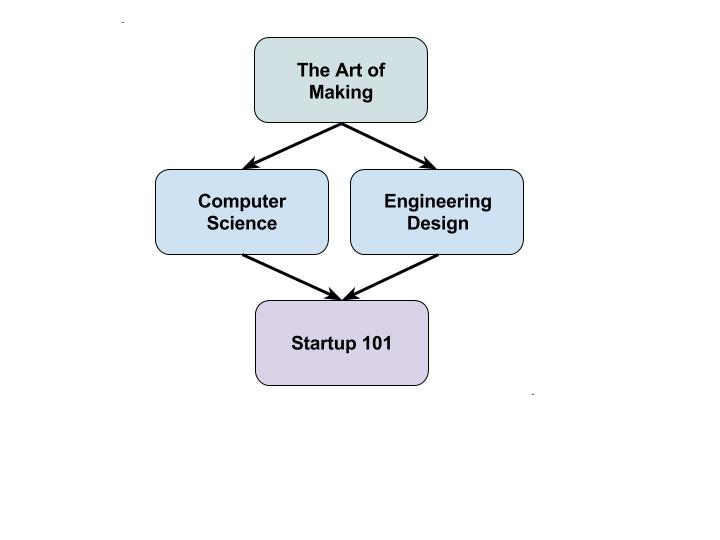
\includegraphics[scale=.5]{CSTiers2.jpg}}
\end{figure}

Potential courses in each track are outlined below.\par
Computer Science
\begin{enumerate}
	\item Creative Coding
	\item Web Design and Development
	\item Software Engineering
\end{enumerate}
Engineering Design
\begin{enumerate}
	\item 3D Art and Design / Tech Theater / Environmental Engineering Design 
	\item Industrial Design
	\item Robotic Systems
\end{enumerate}	

Finally, the tracks reconverge with Startup 101, a course focusing on the ideation, creation, testing, and marketing of unique products and services. The course builds on skills acquired in computer science, engineering, 3D modeling, and design, but adds the element of entrepreneurship. Students will write business models and develop marketing strategies. By the end of the course, students will have an understanding of pathways to innovation, in addition to an understanding of how successful products are launched.\par

\hiddensubsection{Required Exposure}
This document strongly recommends that the Upper School adopt a 1/2 credit CS graduation requirement. A mandated credit, as opposed to an optional elective, ensures that every student---especially groups typically underrepresented in CS---get exposure to coding prior to college. The importance of CS and the dire need for coding experience is explored in Chapter \ref{Introduction}. Of the nine INDEX schools interviewed about CS, the three schools with the most impressive CS programs all had graduation requirements of approximately one semester (refer to Section \ref{index}).\par
That said, there are a few potential problems associated with a graduation requirement. Mandated credits in the Upper School are currently impacting scheduling for certain students; additional requirements would place even greater restrictions on the courses students can take. In addition, a graduation requirement would necessitate the hiring of additional faculty to teach CS courses, which may prove to be difficult. Staffing difficulties, however, should not prevent the enactment of a graduation requirement. The ubiquity of professional development opportunities and online resources should enable non-CS teachers (possibly math or science) to pick up a language. Hiring and training a new teacher, however, may take time.\par
If a required graduation credit is not feasible within a reasonable timeline, mandating CS integration in the Upper School should be considered. Re Each department could be required to expose students to CS through a project at some point during 9th-12th grade, or class deans could be responsible for ensuring that at least one course exposes students to CS each year. Ideally these coding experiences would be scaffolded or coordinated in such a way that students still meet the minimum CS requirements outlined in Appendix \ref{AppendixNEWMAN}. An integration coordinator would be necessary to help non-CS teachers brainstorm and implement project ideas, coordinate between departments and classes to ensure that each class gets necessary exposure to coding, and develop content that meets necessary graduation requirements.\par
The drawbacks and benefits of CS integration are explored in more depth in Section \ref{csint}. One of the primary drawbacks of integration is placing additional burdens on upper school teachers who are already struggling to meeting curriculum requirements. The lack of understanding of CS and the need for professional development is another primary drawback. A integration coordinator, however, may help to mitigate both of these obstacles and would allow all students to get CS exposure without requiring additional graduation requirements.\par

\hiddensubsection{Online Education}
For a full analysis of online platforms, their merits and shortcomings, please refer to \ref{procononline}.\par
There are several examples where online programs add clear value to Newman's CS offerings. Allowing platforms like Global Online Academy or CodeHS to fill niche needs---such as allowing self-directed students to take specific upper level courses---is cost-effective and grants students more options. In addition, using Kahn Academy or other online resources in blended classrooms as a crutch or supplement may bolster in-class instruction.\par
This document, however, does not recommend the strict reliance on online CS platforms, especially for meeting a potential graduation requirement. By the very nature of being ``cookie cutter'' and purely virtual, online platforms cannot offer the same ``rigor and relationships'' as curriculum spearheaded by a teacher. Hooking students, inspiring students, communicating the importance and broad applicability of CS, and ensuring that students recognize the creative and innovative potential of coding---these must be the priorities of a CS program at Newman. CS courses will not compete with other disciplines at Newman without the enthusiasm and relationships created by and with teachers, the personally-relevant curated projects, or the face-to-face communication. In short: Newman is known for its top-notch pedagogy; CS, a critically important field in the 21st century, cannot be the exception. \par
All of that said, hooking students is the priority, after which students may want more freedom to explore advanced topics on their own. Using online CS programs as a second or third tier course may be advisable, but only if resources or hiring difficulties prohibit an in-person CS experience. \par  

\hiddensubsection{Next Steps}
Next year two new courses will be offered in the Makerspace---``The Art of Making'' and ``Creative Coding''---which will lay the groundwork for potential upper school courses in engineering and computer science. Offering these courses as art electives to a small group of students will give time to prototype projects and give insight into the best type of CS instruction that meets the Newman CS benchmarks outlined in \ref{AppendixNEWMAN}. In time, questions related to graduation requirements, additional courses and tiers, offering the AP, and hiring/ staffing needs can be addressed. For now, drumming up student interest and building teacher support is paramount in order to build a sustainable and resilient program.
 
%
\chapter{Conclusion} % Main chapter title

\label{Chapter5} %for referencing this chapter elsewhere, use \ref{ChapterX}

\lhead{\emph{Conclusion}} %this is for the header on each page - perhaps a shortened title



A national review of the status of computer science K-12 education spawns a variety of questions that must be addressed as a CS program develops at Newman. In the Lower School, those questions relate to the balance of coding vs. computer literacy, classroom vs. Media time, physical vs. virtual instruction, and game-based vs. open-ended creative platforms. In the Middle School, which is less amenable to additional electives, the question is: should CS be integrated into the classroom or offered as a standalone course? How will we make space for a new ``core'' subject in an already tight schedule? And for the Upper School, the questions relate to curriculum---should Newman offer an academic approach to CS akin to an introductory course at the university level, or should an upper school program place greater emphasis on the creative, innovative, and applied coding process from industry and code schools? What are the merits of offering the AP? And finally, can online CS instruction replace classroom instruction? \par
While many of these questions can be debated, the dire need for computer science at Newman cannot. Students are graduating without valuable, marketable, and creative computational thinking skills. If Newman is to remain a competitive, top-notch independent school, it must keep pace with this evolving field.\par
Fortunately, even the independent schools with standout programs---schools like Winchester Thurston and Greenhill---are relatively new to CS. Using nationally established benchmarks (CSTA, ISTE, AP, etc.), learning from the experiences of top tier schools and institutions, and leveraging new tools and technologies, Newman has the ability to craft a holistic K-12 CS plan and establish itself as a local and national leader in computer science education.\par
 
%\input{Chapters/Chapter6} 
%\input{Chapters/Chapter7} 

%----------------------------------------------------------------------------------------
%	THESIS CONTENT - APPENDICES
%----------------------------------------------------------------------------------------

\addtocontents{toc}{\vspace{2em}} % Add a gap in the Contents, for aesthetics

\appendix % Cue to tell LaTeX that the following 'chapters' are Appendices

% Include the appendices of the thesis as separate files from the Appendices folder
% Uncomment the lines as you write the Appendices

% Appendix Template

\chapter{Appendix A: Coding Tools \& Curriculum} % Main appendix title

\label{AppendixA} % Change X to a consecutive letter; for referencing this appendix elsewhere, use \ref{AppendixX}

\lhead{Appendix A. \emph{Coding Tools \& Curriculum}} % Change X to a consecutive letter; this is for the header on each page - perhaps a shortened title

The following table is compiled from EdSurge\cite{edsurgetab} and Code.Org\cite{codeapps}. For full descritions and side-by-side comparisons, visit \href{https://code.org/educate/3rdparty}{Code.org's 3rd Educator Party Resources}.
\footnotesize
\begin{longtable}{p{2cm}p{4cm}p{3cm}p{1.3cm}p{1.3cm}p{1.3cm}}	
\caption{K-12 Coding Tools and Curriculum} \\ \hline
\rowcolor[HTML]{D4DCE7} \textbf{Org} & \textbf{Curriculum} & \textbf{PD} & \textbf{Cost} & \textbf{Self-Guided?} & \textbf{Student Tracking?}  \\ \hline

%-----TABLE CONTENTS---------------------------------------%
\hline
\multicolumn{6}{l}{\cellcolor[HTML]{EFEFEF}\textbf{LOWER SCHOOL}} \\   \hline \hline
\href{http://www.scratchjr.org/index.html}{Scratch Jr.} & An iPad app that introduces coding cocepts through games and visual programming. Assessments and curriculum included. & - & FREE & Y & N \\ \hline
\href{http://scratched.gse.harvard.edu/resources/search/results/taxonomy%3A21%2C28}{ScratchEd} & A 6-unit intro to Scratch, a visual programming language for game creation, animations, and art. & In-person educator meet-ups and online MOOC, FREE & FREE & N & N \\ \hline
\href{https://studio.code.org/}{Code Studio (Code.org)} & 4 courses blend online tutorials with “unplugged” activities & 1-day weekend workshops across the US, FREE & FREE & Y & Y \\ \hline
\href{https://www.pltw.org/}{Project Lead The Way} & 6, 10-hour computer science modules & Face-to-face and online, \$700 for school-level lead teacher & \$750 /school & Y & Y \\ \hline
\href{https://www.tynker.com/}{Tynker} & Inspired by Scratch, Tynker has a dashboard to allow teachers to create a more structured way of teaching code with visual blocks. Includes assessment, classroom management, lesson plans, and a built in tutor. & 2-day PD, \$2000/day + travel & FREE tutorials. \$399 /class, \$2,000 /school & Y & Y \\ \hline
\href{https://www.kodable.com/}{Kodable} & Kodable is a freemium educational iPad game offering a kid-friendly introduction to programming concepts and problem solving. & - & FREE & Y & Y \\ \hline
\href{http://snap.berkeley.edu/}{SNAP!} & SNAP!'s visual blocks (similar to Scratch) support higher level computer science concepts like recursion, procedures, and continuations, SNAP! can work with LEGO Mindstorms NXT. & - & FREE & N & N \\ \hline
\href{https://www.gethopscotch.com/}{Hopscotch} & This free iPad app uses a visual programming language similar to Scratch to help kids learn the basics of programming logic, such as sequencing, loops, variables, functions and conditionals. & - & FREE & N & N \\ \hline 

\\ \hline \hline
\multicolumn{6}{l}{\cellcolor[HTML]{EFEFEF}\textbf{MIDDLE SCHOOL}} \\ \hline \hline

\href{http://www.bootstrapworld.org/}{Bootstrap} & Teach algebra through video-game programming, with a 20-hr module to go alongside or inside a math class & 3-day workshops for schools and districts. Fees range & FREE & N & N \\ \hline
\href{https://codehs.com/}{CodeHS} & Year-long Introduction to Computer Science and AP Computer Science in Java.  & Online PD for teaching intro computer science, 30-40 hour course, \$1000/teacher & FREE Intro; Pro version is \$2000/ section /year & Y & Y \\ \hline
\href{https://code.org/educate}{Code.org} & 20-lesson CS in Algebra and CS in Science modules for math and science classes & In-person and online workshops available to partner districts, FREE, 50\% of teacher stipends covered by Code.org & FREE & Y & Y \\ \hline
\href{http://globaloria.com/courses-services/}{Globaloria} & 6 game-design courses & 3-day, in-person training and ongoing online PD, fee included in student price & \$75 /student & Y & Y \\ \hline
\href{https://www.pltw.org/}{Project Lead The Way} & 6, 10-hour computer science modules & Face-to-face and online, \$700 for school-level lead teacher & \$750 /school & Y & Y \\ \hline
\href{http://scratched.gse.harvard.edu/resources/search/results/taxonomy%3A21%2C28}{ScratchEd} & A 6-unit intro to Scratch & In-person educator meet-ups and online MOOC, FREE & FREE & N & N \\ \hline
\href{https://www.tynker.com/}{Tynker} & Inspired by Scratch, Tynker has a dashboard to allow teachers to create a more structured way of teaching code with visual blocks. Includes assessment, classroom management, lesson plans, and a built in tutor. & 2-day PD, \$2000/day + travel & Free tutorials. \$399 /class, \$2,000 /school & Y & Y \\ \hline
\href{http://snap.berkeley.edu/}{SNAP!} & SNAP!'s visual blocks (similar to Scratch) support higher level computer science concepts like recursion, procedures, and continuations, SNAP! can work with LEGO Mindstorms NXT. & See Scratch & FREE & N & N \\ \hline
\href{https://nclab.com/karel/}{NCLab} & Courses in Karel coding, Turtle coding, 3D modeling, and Python. & Online & \$899 /class & Y & Y \\ \hline
\href{http://app.pluralsight.com/training/player?author=joe-hummel&name=learning-programming-scratch-m0-installation-windows&mode=live&clip=0&course=learning-programming-scratch}{Pluaralsight} & Free video-led coding courses for kids on Scratch, HTML, App Inventor, Kodu and Hopscotch & Online & FREE & Y & N \\ \hline

\\ \hline \hline
\multicolumn{6}{l}{\cellcolor[HTML]{EFEFEF}\textbf{UPPER SCHOOL}} \\ \hline \hline

\href{http://bjc.berkeley.edu/}{Beauty and Joy of Computing} & Year-long CS Principles course & In-person in NYC, Berkeley, CA and North Carolina, FREE, stipends in NYC, stipends + travel elsewhere paid as available & FREE & N & N \\ \hline
\href{http://www.bootstrapworld.org/}{Bootstrap} & Teach algebra through video-game programming, with a 20-hr module to go alongside or inside a math class & 3-day workshops for schools and districts. Fees range & FREE & N & N \\ \hline
\href{https://www.codecademy.com/learn}{Codecademy} & 6 online courses (Javascript, SQL, Python, Ruby on Rails, Git, HTML/CSS, and more) and 65 projects. FREE & Not provided & FREE & Y & Y \\ \hline
\href{https://codehs.com/}{CodeHS} & Year-long Introduction to Computer Science and AP Computer Science in Java.  & Online PD for teaching intro computer science, 30-40 hour course, \$1000/teacher & FREE Intro; Pro version is \$2000/section/year & Y & Y \\ \hline
\href{https://code.org/educate}{Code.org} & Exploring Computer Science intro course and Computer Science Principles, a pilot course with an AP exam coming in 2016 & In-person and online workshops available to partner districts, FREE, 50\% of teacher stipends covered by Code.org & FREE & N & N \\ \hline
\href{https://edhesive.com/}{Edhesive} & Year-long AP Computer Science course & Online PD, community and content/technical/program support available, \$2,200 per school & FREE & Y & Y \\ \hline
\href{http://globaloria.com/courses-services/}{Globaloria} & 6 game-design courses & 3-day, in-person training and ongoing online PD, fee included in student price & \$75/student & Y & Y \\ \hline
\href{https://ram8647.appspot.com/mobileCSP/}{Mobile CSP} & Year-long AP Computer Science Principles course based on App Inventor, a mobile programming language for Android devices. Materials available online & Online, regional in-person offered in CT, MA, NH and CA (others may be available), FREE, stipends available & FREE & Y & N \\ \hline
\href{https://www.pltw.org/faq/computer-science}{Project Lead The Way} & Several courses: Intro CS, AP, Cybersecurity, and CS Applications & 5 or 10-day in-person training, \$1200 or \$2400, depending on course & \$2000 /school & Y & Y \\ \hline
\href{https://www.khanacademy.org/computing/computer-science}{Khan Academy} & Online curriculum that teaches JavaScript programming, HTML/CSS, and SQL, in an interactive online environment, plus courses on Algorithms and Cryptography.  & Online & FREE & Y & Y \\ \hline
\href{https://nclab.com/karel/}{NCLab} & Courses in Karel coding, Turtle coding, 3D modeling, and Python. & Online & \$899 /class & Y & Y \\ \hline
\href{http://hello.processing.org/}{Hello Processing} & Video tutorials and interactive coding environment for learning Processing. & Online & FREE & Y & N \\ \hline
\href{https://www.codeavengers.com/teacher/info}{Code Avengers} & In-browser exercises and courses in JavaScript, HTML5, CSS3 and Python. Introductory courses are free, with intermediate and advanced courses for $29-$39.  & Online & FREE intro; intermediate and advanced courses for \$29-\$39.  & Y & Y \\ \hline
\end{longtable}	

---


%% Appendix Template

\chapter{Appendix B: Hardware Tools} % Main appendix title

\label{AppendixB} % Change X to a consecutive letter; for referencing this appendix elsewhere, use \ref{AppendixX}

\lhead{Appendix B. \emph{Physical Computing Tools}} % Change X to a consecutive letter; this is for the header on each page - perhaps a shortened title

physical computing
Arduino 
Raspberri Pi
Android Robotics

Sphero
LEGO Robotics



LittleBits (?)
Makey Makey + Scratch



---


%% Appendix C

\chapter{Appendix C: CSTA Benchmarks} % Main appendix title

\label{AppendixCSTA} % For referencing this appendix elsewhere, use \ref{AppendixA}

\lhead{Appendix C. \emph{CSTA Benchmarks}} % This is for the header on each page - perhaps a shortened title
% Please add the following required packages to your document preamble:
% \usepackage[normalem]{ulem}
% \useunder{\uline}{\ul}{}
The Computer Science Teachers Association (CSTA) K-12 Computer Science Standards (revised 2011) ~\cite{csta} are broken into tables by level: K-3rd grade, 3rd-6th grade, level 2 (i.e. introductory high school sequence), level 3A, and level 3B. The benchmark subject areas include collaboration, computers and communication devices, computational thinking, community and ethical impacts, and computing practice and programming. \par 
\begin{longtable}{p{1.8cm}p{11cm}}
\caption{K-3rd Grade CS Benchmarks} \\
\textbf{ID} & \textbf{DESCRIPTION} \\ \hline
\multicolumn{2}{c}{\textit{COLLABORATION}} \\
 L0C01   & Gather information and communicate electronically with others with support from teachers, family members, or student partners.                                                                                             \\
 L0C02   & Work cooperatively and collaboratively with peers, teachers, and others using technology                                                                                                                                   \\
 \multicolumn{2}{c}{\textit{COMPUTERS AND COMMUNICATION DEVICES}}                                                     \\
 L0CD01  & Use standard input and output devices to successfully operate computers and related technologies.                                                                                                                          \\
 \multicolumn{2}{c}{\textit{COMPUTING PRACTICE AND PROGRAMMING}}                                                                                                                                                                                     \\
 L0CP01  & Use technology resources to conduct age-appropriate research.                                                                                                                                                              \\
 L0CP02  & Use developmentally appropriate multimedia resources (e.g., interactive books and educational software) to support learning across the curriculum.                                                                         \\
 L0CP03  & Create developmentally appropriate multimedia products with support from teachers, family members, or student partners.                                                                                                    \\
 L0CP04  & Construct a set of statements to be acted out to accomplish a simple task (e.g., turtle instructions).                                                                                                                     \\
 L0CP05  & Identify jobs that use computing and technology.                                                                                                                                                                           \\
 L0CP06  & Gather and organize information using concept-mapping tools.                                                                                                                                                               \\
 \multicolumn{2}{c}{\textit{COMPUTATIONAL THINKING}}                                                     
 \\
 L0CT01  & Use technology resources (e.g., puzzles, logical thinking programs) to solve ageappropriate problems                                                                                                                       \\
 L0CT02  & Use writing tools, digital cameras, and drawing tools to illustrate thoughts, ideas, and stories in a step-by-step manner.                                                                                                 \\
 L0CT03  & Understand how to arrange (sort) information into useful order, such as sorting students by birth date, without using a computer.                                                                                          \\
 L0CT04  & Recognize that software is created to control computer operations.                                                                                                                                                         \\
 L0CT05  & Demonstrate how 0s and 1s can be used to represent information.                                                   
\end{longtable}																												

\begin{longtable}{p{1.8cm}p{11cm}}
\caption{3rd-6th Grade CS Benchmarks} \\
\textbf{ID} & \textbf{DESCRIPTION} \\ \hline
\multicolumn{2}{c}{\textit{COLLABORATION}} \\
 L1C01   & Use productivity technology tools (e.g., word processing, spreadsheet, presentation software) for individual and collaborative writing, communication, and publishing activities.                                          \\
 L1C02   & Use online resources (e.g., email, online discussions, collaborative web environments) to participate in collaborative problemsolving activities for the purpose of developing solutions or products.                      \\
 L1C03   & Identify ways that teamwork and collaboration can support problem solving and innovation.                                                                                                                                  \\
 \multicolumn{2}{c}{\textit{COMPUTERS AND COMMUNICATION DEVICES}}                                                                                                                                                                                   \\
 L1CD1   & Demonstrate an appropriate level of proficiency with keyboards and other input and output devices                                                                                                                          \\
 L1CD2   & Understand the pervasiveness of computers and computing in daily life (e.g., voice mail, downloading videos and audio files, microwave ovens, thermostats, wireless Internet, mobile computing devices, GPS systems).      \\
 L1CD3   & Apply strategies for identifying simple hardware and software problems that may occur during use.                                                                                                                          \\
 L1CD4   & Identify that information is coming to the computer from many sources over a network.                                                                                                                                      \\
 L1CD5   & Identify factors that distinguish humans from machines.                                                                                                                                                                    \\
 L1CD6   & Recognize that computers model intelligent behavior (as found in robotics, speech and language recognition, and computer animation).                                                                                       \\
 \multicolumn{2}{c}{\textit{COMMUNITY, GLOBAL, AND ETHICAL IMPACTS}}                                                                                                                                                                                \\
 L1CI01  & Discuss basic issues related to responsible use of technology and information, and the consequences of inappropriate use.                                                                                                  \\
 L1CI02  & Identify the impact of technology (e.g., social networking, cyber bullying, mobile computing and communication, web technologies, cyber security, and virtualization) on personal life and society.                        \\
 L1CI03  & Evaluate the accuracy, relevance, appropriateness, comprehensiveness, and biases that occur in electronic information sources.                                                                                             \\
 L1CI04  & Understand ethical issues that relate to computers and networks (e.g., equity of access, security, privacy, copyright, and intellectual property).                                                                         \\
 \multicolumn{2}{c}{\textit{COMPUTING PRACTICE AND PROGRAMMING}}                                                                                                                                                                                         \\
 L1CP01  & Use technology resources (e.g., calculators, data collection probes, mobile devices, videos, educational software, and web tools) for problem-solving and self-directed learning.                                          \\
 L1CP02  & Use general-purpose productivity tools and peripherals to support personal productivity, remediate skill deficits, and facilitate learning.                                                                                \\
 L1CP03  & Use technology tools (e.g., multimedia and text authoring, presentation, web tools, digital cameras, and scanners) for individual and collaborative writing, communication, and publishing activities.                     \\
 L1CP04  & Gather and manipulate data using a variety of digital tools.                                                                                                                                                               \\
 L1CP05  & Construct a program as a set of step-by-step instructions to be acted out (e.g., make a peanut butter and jelly sandwich activity).                                                                                        \\
 L1CP06  & Implement problem solutions using a blockbased visual programming language.                                                                                                                                                \\
 L1CP07  & Use computing devices to access remote information, communicate with others in support of direct and independent learning, and pursue personal interests.                                                                  \\
 L1CP08  & Navigate between webpages using hyperlinks and conduct simple searches using search engines.                                                                                                                               \\
 L1CP09  & Identify a wide range of jobs that require knowledge or use of computing.                                                                                                                                                  \\
 L1CP10  & Gather and manipulate data using a variety of digital tools.                                                                                                                                                               \\
 \multicolumn{2}{c}{\textit{COMPUTATIONAL THINKING}}                                                                                                                                                                                                     \\
 L1CT01  & Understand and use the basic steps in algorithmic problem-solving (e.g., problem statement and exploration, examination of sample instances, design, implementation, and testing).                                         \\
 L1CT02  & Develop a simple understanding of an algorithm (e.g., search, sequence of events, or sorting) using computer-free exercises.                                                                                               \\
 L1CT03  & Demonstrate how a string of bits can be used to represent alphanumeric information.                                                                                                                                        \\
 L1CT04  & Describe how a simulation can be used to solve a problem.                                                                                                                                                                  \\
 L1CT05  & Make a list of sub-problems to consider while addressing a larger problem.                                                                                                                                                 \\
 L1CT06  & Understand the connections between computer science and other fields.                                                                                                                                                      \\
\end{longtable}	
\begin{longtable}{p{1.8cm}p{11cm}}
\caption{Level 2 CS Benchmarks} \\
\textbf{ID} & \textbf{DESCRIPTION} \\ \hline
\multicolumn{2}{c}{\textit{COLLABORATION}} \\
 L2C01   & Apply productivity/multimedia tools and peripherals to group collaboration and support learning throughout the curriculum.                                                                                                 \\
 L2C02   & Collaboratively design, develop, publish, and present products (e.g., videos, podcasts, websites) using technology resources that demonstrate and communicate curriculum concepts.                                         \\
 L2C03   & Collaborate with peers, experts, and others using collaborative practices such as pair programming, working in project teams, and participating in group active learning activities.                                       \\
 L2C04   & Exhibit dispositions necessary for collaboration: providing useful feedback, integrating feedback, understanding and accepting multiple perspectives, socialization.                                                       \\
 \multicolumn{2}{c}{\textit{COMPUTERS AND COMMUNICATION DEVICES}}                                                                                                                                                                                   \\
 L2CD01  & Recognize that computers are devices that execute programs.                                                                                                                                                                \\
 L2CD02  & Identify a variety of electronic devices that contain computational processors.                                                                                                                                            \\
 L2CD03  & Demonstrate an understanding of the relationship between hardware and software.                                                                                                                                            \\
 L2CD04  & Use developmentally appropriate, accurate terminology when communicating about technology.                                                                                                                                 \\
 L2CD05  & Apply strategies for identifying and solving routine hardware problems that occur during everyday computer use.                                                                                                            \\
 L2CD06  & Describe the major components and functions of computer systems and networks.                                                                                                                                              \\
 L2CD07  & Describe what distinguishes humans from machines focusing on human intelligence versus machine intelligence and ways we can communicate.                                                                                   \\
 L2CD08  & Describe ways in which computers use models of intelligent behavior (e.g., robot motion, speech and language understanding, and computer vision).                                                                          \\
 \multicolumn{2}{c}{\textit{COMMUNITY, GLOBAL, AND ETHICAL IMPACTS}}                                                                                                                                                                                 \\
 L2CI01  & Exhibit legal and ethical behaviors when using information and technology and discuss the consequences of misuse.                                                                                                          \\
 L2CI02  & Demonstrate knowledge of changes in information technologies over time and the effects those changes have on education, the workplace, and society.                                                                        \\
 L2CI03  & Analyze the positive and negative impacts of computing on human culture.                                                                                                                                                   \\
 L2CI04  & Evaluate the accuracy, relevance, appropriateness, comprehensiveness, and bias of electronic information sources concerning real-world problems.                                                                           \\
 L2CI05  & Describe ethical issues that relate to computers and networks (e.g., security, privacy, ownership, and information sharing).                                                                                               \\
 L2CI06  & Discuss how the unequal distribution of computing resources in a global economy raises issues of equity, access, and power.                                                                                                \\
 \multicolumn{2}{c}{\textit{COMPUTING PRACTICE AND PROGRAMMING}}                                                                                                                                                                                          \\
 L2CP01  & Select appropriate tools and technology resources to accomplish a variety of tasks and solve problems.                                                                                                                     \\
 L2CP02  & Use a variety of multimedia tools and peripherals to support personal productivity and learning throughout the curriculum.                                                                                                 \\
 L2CP03  & Design, develop, publish, and present products (e.g., webpages, mobile applications, animations) using technology resources that demonstrate and communicate curriculum concepts.                                          \\
 L2CP04  & Demonstrate an understanding of algorithms and their practical application.                                                                                                                                                \\
 L2CP05  & Implement problem solutions using a programming language, including: looping behavior, conditional statements, logic, expressions, variables, and functions.                                                               \\
 L2CP06  & Demonstrate good practices in personal information security, using passwords, encryption, and secure transactions.                                                                                                         \\
 L2CP07  & Identify interdisciplinary careers that are enhanced by computer science.                                                                                                                                                  \\
 L2CP08  & Demonstrate dispositions amenable to openended problem solving and programming (e.g., comfort with complexity, persistence, brainstorming, adaptability, patience, propensity to tinker, creativity, accepting challenge). \\
 L2CP09  & Collect and analyze data that is output from multiple runs of a computer program.                                                                                                                                          \\
 \multicolumn{2}{c}{\textit{COMPUTATIONAL THINKING}}                                                                                                                                                                                                     \\
 L2CT01  & Use the basic steps in algorithmic problemsolving to design solutions (e.g., problem statement and exploration, examination of sample instances, design, implementing a solution, testing, evaluation).                    \\
 L2CT02  & Describe the process of parallelization as it relates to problem solving.                                                                                                                                                  \\
 L2CT03  & Define an algorithm as a sequence of instructions that can be processed by a computer.                                                                                                                                     \\
 L2CT04  & Evaluate ways that different algorithms may be used to solve the same problem.                                                                                                                                             \\
 L2CT05  & Act out searching and sorting algorithms.                                                                                                                                                                                  \\
 L2CT06  & Describe and analyze a sequence of instructions being followed (e.g., describe a character’s behavior in a video game as driven by rules and algorithms).                                                                  \\
 L2CT07  & Represent data in a variety of ways including text, sounds, pictures, and numbers.                                                                                                                                         \\
  L2CT08  & Use visual representations of problem states, structures, and data (e.g., graphs, charts, network diagrams, flowcharts).    \\
 L2CT09  & Interact with content-specific models and simulations (e.g., ecosystems, epidemics, molecular dynamics) to support learning and research.                                                                                  \\
 L2CT10  & Evaluate what kinds of problems can be solved using modeling and simulation.                                                                                                                                               \\
 L2CT11  & Analyze the degree to which a computer model accurately represents the real world.                                                                                                                                         \\
 L2CT12  & Use abstraction to decompose a problem into sub problems.                                                                                                                                                                  \\
 L2CT13  & Understand the notion of hierarchy and abstraction in computing including highlevel languages, translation, instruction set, and logic circuits.                                                                           \\
 L2CT14  & Examine connections between elements of mathematics and computer science including binary numbers, logic, sets and functions.                                                                                              \\
 L2CT15  & Provide examples of interdisciplinary applications of computational thinking.                                                                                                                                              \\

\end{longtable}                                                                                               
\begin{longtable}{p{1.8cm}p{11cm}}
\caption{Level 3A CS Benchmarks} \\
\textbf{ID} & \textbf{DESCRIPTION} \\ \hline
\multicolumn{2}{c}{\textit{COLLABORATION}} \\
 L3AC01  & Work in a team to design and develop a software artifact.                                                                                                                                                                  \\
 L3AC02  & Use collaborative tools to communicate with project team members (e.g., discussion threads, wikis, blogs, version control, etc.).                                                                                          \\
 L3AC03  & Describe how computing enhances traditional forms and enables new forms of experience, expression, communication, and collaboration                                                                                        \\
 L3AC04  & Identify how collaboration influences the design and development of software products.                                                                                                                                     \\
 \multicolumn{2}{c}{\textit{COMPUTERS AND COMMUNICATION DEVICES}}                                                                                                                                                                                   \\
 L3ACD01 & Describe the unique features of computers embedded in mobile devices and vehicles (e.g., cell phones, automobiles, airplanes).                                                                                             \\
 L3ACD02 & Develop criteria for purchasing or upgrading computer system hardware.                                                                                                                                                     \\
 L3ACD03 & Describe the principal components of computer organization (e.g., input, output, processing, and storage).                                                                                                                 \\
 L3ACD04 & Compare various forms of input and output.                                                                                                                                                                                 \\
 L3ACD05 & Explain the multiple levels of hardware and software that support program execution (e.g., compilers, interpreters, operating systems, networks).                                                                          \\
 L3ACD06 & Apply strategies for identifying and solving routine hardware and software problems that occur in everyday life.                                                                                                           \\
 L3ACD07 & Compare and contrast client-server and peer-to-peer network strategies.                                                                                                                                                    \\
 L3ACD08 & Explain the basic components of computer networks (e.g., servers, file protection, routing, spoolers and queues, shared resources, and fault-tolerance).                                                                   \\
 L3ACD09 & Describe how the Internet facilitates global communication.                                                                                                                                                                \\
 L3ACD10 & Describe the major applications of artificial intelligence and robotics.                                                                                                                                                   \\
 \multicolumn{2}{c}{\textit{COMMUNITY, GLOBAL, AND ETHICAL IMPACTS}}                                                                                                                                                                                 \\
 L3ACI01 & Compare appropriate and inappropriate social networking behaviors.                                                                                                                                                         \\
 L3ACI02 & Discuss the impact of computing technology on business and commerce (e.g., automated tracking of goods, automated financial transactions, e-commerce, cloud computing).                                                    \\
 L3ACI03 & Describe the role that adaptive technology can play in the lives of people with special needs.                                                                                                                             \\
 L3ACI04 & Compare the positive and negative impacts of technology on culture (e.g., social networking, delivery of news and other public media, and intercultural communication).                                                    \\
 L3ACI05 & Describe strategies for determining the reliability of information found on the Internet.                                                                                                                                  \\
 L3ACI06 & Differentiate between information access and information distribution rights.                                                                                                                                              \\
 L3ACI07 & Describe how different kinds of software licenses can be used to share and protect intellectual property.                                                                                                                  \\
 L3ACI08 & Discuss the social and economic implications associated with hacking and software piracy.                                                                                                                                  \\
 L3ACI09 & Describe different ways in which software is created and shared and their benefits and drawbacks (commercial software, public domain software, open source development).                                                   \\
 L3ACI10 & Describe security and privacy issues that relate to computer networks.                                                                                                                                                     \\
 L3ACI11 & Explain the impact of the digital divide on access to critical information.                                                                                                                                                \\
 \multicolumn{2}{c}{\textit{COMPUTING PRACTICE AND PROGRAMMING}}                                                                                                                                                                                        \\
 L3ACP01 & Create and organize Web pages through the use of a variety of web programming design tools.                                                                                                                                \\
 L3ACP02 & Use mobile devices/emulators to design, develop, and implement mobile computing applications.                                                                                                                              \\
 L3ACP03 & Use various debugging and testing methods to ensure program correctness (e.g., test cases, unit testing, white box, black box, integration testing)                                                                        \\
 L3ACP04 & Apply analysis, design, and implementation techniques to solve problems (e.g., use one or more software lifecycle models).                                                                                                 \\
 L3ACP05 & Use Application Program Interfaces (APIs) and libraries to facilitate programming solutions.                                                                                                                               \\
 L3ACP06 & Select appropriate file formats for various types and uses of data.                                                                                                                                                        \\
 L3ACP07 & Describe a variety of programming languages available to solve problems and develop systems.                                                                                                                               \\
 L3ACP08 & Explain the program execution process.                                                                                                                                                                                     \\
 L3ACP09 & Explain the principles of security by examining encryption, cryptography, and authentication techniques.                                                                                                                   \\
 L3ACP10 & Explore a variety of careers to which computing is central.                                                                                                                                                                \\
 L3ACP11 & Describe techniques for locating and collecting small and large-scale data sets.                                                                                                                                           \\
 L3ACP12 & Describe how mathematical and statistical functions, sets, and logic are used in computation.                                                                                                                              \\
 \multicolumn{2}{c}{\textit{COMPUTATIONAL THINKING}}                                                                                                                                                                                                     \\
 L3ACT01 & Use predefined functions and parameters, classes and methods to divide a complex problem into simpler parts.                                                                                                               \\
 L3ACT02 & Describe a software development process used to solve software problems (e.g., design, coding, testing, verification).                                                                                                     \\
 L3ACT03 & Explain how sequence, selection, iteration, and recursion are building blocks of algorithms.                                                                                                                               \\
 L3ACT04 & Compare techniques for analyzing massive data collections.                                                                                                                                                                 \\
 L3ACT05 & Describe the relationship between binary and hexadecimal representations.                                                                                                                                                  \\
 L3ACT06 & Analyze the representation and trade-offs among various forms of digital information.                                                                                                                                      \\
 L3ACT07 & Describe how various types of data are stored in a computer system.                                                                                                                                                        \\
 L3ACT08 & Use modeling and simulation to represent and understand natural phenomena.                                                                                                                                                 \\
 L3ACT09 & Discuss the value of abstraction to manage problem complexity.                                                                                                                                                             \\
 L3ACT10 & Describe the concept of parallel processing as a strategy to solve large problems.                                                                                                                                         \\
 L3ACT11 & Describe how computation shares features with art and music by translating human intention into an artifact.                                                                                                               \\
\end{longtable}                                                                                               
\begin{longtable}{p{1.8cm}p{11cm}}
\caption{Level 3B CS Benchmarks} \\
\textbf{ID} & \textbf{DESCRIPTION} \\ \hline
\multicolumn{2}{c}{\textit{COLLABORATION}} \\
 L3BC01  & Use project collaboration tools, version control systems, and Integrated Development Environments (IDEs) while working on a collaborative software project.                                                                \\
 L3BC02  & Demonstrate the software life cycle process by participating on a software project team.                                                                                                                                   \\
 L3BC03  & Evaluate programs written by others for readability and usability                                                                                                                                                          \\
 \multicolumn{2}{c}{\textit{COMPUTERS AND COMMUNICATION DEVICES}}                                                                                                                                                                                 \\
 L3BCD01 & Discuss the impact of modifications on the functionality of application programs.                                                                                                                                          \\
 L3BCD02 & Identify and describe hardware (e.g., physical layers, logic gates, chips, components).                                                                                                                                    \\
 L3BCD03 & Identify and select the most appropriate file format based on trade-offs (e.g., accuracy, speed, ease of manipulation).                                                                                                    \\
 L3BCD04 & Describe the issues that impact network functionality (e.g., latency, bandwidth, firewalls, server capability).                                                                                                            \\
 L3BCD05 & Explain the notion of intelligent behavior through computer modeling and robotics.                                                                                                                                         \\
 \multicolumn{2}{c}{\textit{COMMUNITY, GLOBAL, AND ETHICAL IMPACTS}}                                                                                                                                                                                \\
 L3BCI01 & Demonstrate ethical use of modern communication media and devices.                                                                                                                                                         \\
 L3BCI02 & Analyze the beneficial and harmful effects of computing innovations.                                                                                                                                                       \\
 L3BCI03 & Summarize how financial markets, transactions, and predictions have been transformed by automation.                                                                                                                        \\
 L3BCI04 & Summarize how computation has revolutionized the way people build real and virtual organizations and infrastructures.                                                                                                      \\
 L3BCI05 & Identify laws and regulations that impact the development and use of software.                                                                                                                                             \\
 L3BCI06 & Analyze the impact of government regulation on privacy and security.                                                                                                                                                       \\
 L3BCI07 & Differentiate among open source, freeware, and proprietary software licenses and their applicability to different types of software.                                                                                       \\
 L3BCI08 & Relate issues of equity, access, and power to the distribution of computing resources in a global society.                                                                                                                 \\
 \multicolumn{2}{c}{\textit{COMPUTING PRACTICE AND PROGRAMMING}}                                                                                                                                                                                        \\
 L3BCP01 & Use advanced tools to create digital artifacts (e.g., web design, animation, video, multimedia)                                                                                                                            \\
 L3BCP02 & Use tools of abstraction to decompose a large-scale computational problem (e.g., procedural abstraction, object-oriented design, functional design).                                                                       \\
 L3BCP03 & Classify programming languages based on their level and application domain                                                                                                                                                 \\
 L3BCP04 & Explore principles of system design in scaling, efficiency, and security.                                                                                                                                                  \\
 L3BCP05 & Deploy principles of security by implementing encryption and authentication strategies.                                                                                                                                    \\
 L3BCP06 & Anticipate future careers and the technologies that will exist.                                                                                                                                                            \\
 L3BCP07 & Use data analysis to enhance understanding of complex natural and human systems.                                                                                                                                           \\
 L3BCP08 & Deploy various data collection techniques for different types of problems.                                                                                                                                                 \\
 \multicolumn{2}{c}{\textit{COMPUTATIONAL THINKING}}                                                                                                                                                                                                     \\
 L3BCT01 & Classify problems as tractable, intractable, or computationally unsolvable.                                                                                                                                                \\
 L3BCT02 & Explain the value of heuristic algorithms to approximate solutions for intractable problems.                                                                                                                               \\
 L3BCT03 & Critically examine classical algorithms and implement an original algorithm.                                                                                                                                               \\
 L3BCT04 & Evaluate algorithms by their efficiency, correctness, and clarity.                                                                                                                                                         \\
 L3BCT05 & Use data analysis to enhance understanding of complex natural and human systems.                                                                                                                                           \\
 L3BCT06 & Compare and contrast simple data structures and their uses (e.g., arrays and lists).                                                                                                                                       \\
 L3BCT07 & Discuss the interpretation of binary sequences in a variety of forms (e.g., instructions, numbers, text, sound, image).                                                                                                    \\
 L3BCT08 & Use models and simulations to help formulate, refine, and test scientific hypotheses.                                                                                                                                      \\
 L3BCT09 & Analyze data and identify patterns through modeling and simulation.                                                                                                                                                        \\
 L3BCT10 & Decompose a problem by defining new functions and classes.                                                                                                                                                                 \\
 L3BCT11 & Demonstrate concurrency by separating processes into threads and dividing data into parallel streams.
\end{longtable}

\addtocontents{toc}{\vspace{2em}} % Add a gap in the Contents, for aesthetics

\backmatter

%----------------------------------------------------------------------------------------
%	BIBLIOGRAPHY
%----------------------------------------------------------------------------------------

\label{Bibliography}

\lhead{\emph{Bibliography}} % Change the page header to say "Bibliography"

\bibliographystyle{unsrtnat} % Use the "unsrtnat" BibTeX style for formatting the Bibliography

\bibliography{Bibliography} % The references (bibliography) information are stored in the file named "Bibliography.bib"

\end{document}  